\documentclass[10pt,twocolumn]{article}

% ===== packages =====
\usepackage[a4paper,margin=0.75in,columnsep=0.55cm]{geometry}
\usepackage[utf8]{inputenc}
\usepackage[T1]{fontenc}
\usepackage{lmodern}
\usepackage{microtype}
\usepackage{amsmath,amssymb}
\usepackage{graphicx}
\usepackage{tikz}
\usetikzlibrary{positioning,arrows.meta,calc,shapes.geometric,backgrounds,fit}
\usepackage{booktabs}
\usepackage{array}
\usepackage{tabularx}
\usepackage{xcolor}
\usepackage{enumitem}
\usepackage[round]{natbib}
\usepackage{titlesec}
\usepackage[hidelinks]{hyperref}

% ===== light styling =====
\definecolor{legalblue}{RGB}{20,60,120}
\titleformat{\section}{\normalfont\large\bfseries\color{legalblue}}{\thesection}{0.6em}{}
\titleformat{\subsection}{\normalfont\normalsize\bfseries}{\thesubsection}{0.6em}{}
\setlength{\parskip}{0pt}
\setlength{\parindent}{1.1em}
\emergencystretch=2em
\renewcommand{\arraystretch}{1.25}
\hypersetup{colorlinks=true, linkcolor=legalblue, citecolor=legalblue, urlcolor=legalblue}

% ===== float tuning (many wide tables) =====
\setcounter{topnumber}{3}
\setcounter{totalnumber}{5}
\renewcommand{\topfraction}{0.95}
\renewcommand{\bottomfraction}{0.9}
\renewcommand{\textfraction}{0.05}
\renewcommand{\floatpagefraction}{0.8}

% ===== title =====
\title{\textbf{Legal AI: From Case-Based Reasoning to Reliable, Structure-Aware Retrieval-Augmented Generation}}
\author{Ali Hamza\\[2pt]
\small Department of Software Engineering, Military College of Signals (MCS),\\
\small National University of Sciences and Technology (NUST), Islamabad, Pakistan\\
\small \texttt{ahamza.msse25mcs@student.nust.edu.pk}}
\date{\today}

\begin{document}
\twocolumn[
\begin{@twocolumnfalse}
\maketitle

\begin{abstract}
\noindent
Legal work depends on finding, interpreting, and applying authoritative texts. Lawyers
and judges work with statutes, regulations, prior decisions, and procedural rules. A
useful AI system must therefore do more than produce fluent language: it must connect its
claims to relevant and reliable legal sources. This survey traces the development of legal
artificial intelligence from case-based reasoning in the early 1990s to contemporary legal
language models and retrieval-augmented generation (RAG). Rather than presenting a simple
chronology, we explain how each wave of methods responded to limitations in earlier
approaches. We review foundational reasoning systems, legal language models, benchmarks,
legal information retrieval, RAG, and studies of hallucination and citation reliability. We
then examine three recent system designs that improve different parts of the pipeline:
document drafting with RAG, fine-tuning of retrieval and generation, and structure-aware
indexing. The review highlights persistent challenges in statutory hierarchy preservation,
citation verification, multilingual access, and jurisdictional coverage, with particular
attention to under-represented legal systems such as Pakistan. We distinguish findings
reported by the original authors from limitations inferred from a study's scope or
evaluation.
\end{abstract}
\vspace{1.2em}
\end{@twocolumnfalse}
]

\section{Introduction}
\label{sec:intro}

Law is a domain in which the quality of an answer depends not only on whether it sounds
reasonable, but also on whether it is supported by the correct legal authority. A useful legal
information system must identify relevant statutes and precedents, interpret them in context,
account for their relationships, and present conclusions that can be checked against
authoritative sources. These requirements make legal artificial intelligence (LegalAI) a
distinctive research challenge. Unlike many general question-answering tasks, legal information
retrieval can depend on exact statutory language, the relationship between a provision and its
subordinate clauses, the authority of a judicial decision, and the jurisdiction and date to
which a legal rule applies. A response that overlooks one of these conditions may appear
convincing while remaining legally incomplete or incorrect.

The effort to automate legal reasoning predates modern machine learning. Early research explored
how computational systems could represent legal rules, compare cases, and construct arguments
resembling those used by lawyers. Ashley's work on case-based reasoning, including HYPO,
demonstrated how a system could reason about legal disputes by comparing fact patterns and
identifying legally meaningful similarities and differences \citep{ashley1991}. This tradition
established an important principle: legal reasoning cannot always be reduced to matching a
question with a sentence. It often requires identifying which facts matter, which rules apply,
and why one authority supports an argument more strongly than another. However, rule-based and
case-based approaches also faced practical constraints. Their performance depended on how legal
knowledge was represented, how exceptions and changing authorities were handled, and how much
domain-specific knowledge could be encoded and maintained.

The growth of statistical natural language processing and pretrained language models changed how
researchers approached these problems. Rather than relying exclusively on manually encoded rules,
machine-learning systems began to learn linguistic patterns from legal documents and perform
tasks such as document classification, information extraction, and case retrieval. Domain-adapted
models such as LEGAL-BERT illustrated the value of training language representations on legal text
rather than relying only on general-purpose language data \citep{chalkidis2020}. Benchmarks such
as LexGLUE and LegalBench subsequently provided more systematic ways to evaluate legal language
models across different tasks and forms of legal reasoning \citep{chalkidis2022, guha2023}. These
developments helped move LegalAI from narrowly engineered expert systems toward more flexible,
data-driven models.

The arrival of large language models (LLMs) expanded these capabilities further. Modern models can
summarize legal documents, explain provisions in natural language, compare arguments, and draft
responses to complex questions. Yet fluency introduces a serious reliability problem. A model may
generate an answer that is coherent and professionally written without accurately reflecting the
law, may cite a nonexistent authority, or may combine correct legal statements in a way that
produces an unsupported conclusion. Research on legal hallucinations has shown why apparent
linguistic quality cannot be treated as evidence of legal correctness \citep{dahl2024,
magesh2025}. In legal practice, this distinction is particularly important because users need to
verify not only the answer, but also the authorities and reasoning on which it depends.

Retrieval-augmented generation (RAG) offers one response to this challenge. Instead of asking an
LLM to answer exclusively from its learned parameters, a RAG system retrieves external documents
and supplies their content as evidence for answer generation. This design can make legal answers
more current, traceable, and specific to an authoritative corpus. However, retrieval does not
automatically guarantee correctness. If a system retrieves an irrelevant judgment, misses a
decisive statutory exception, or separates a provision from its legal hierarchy, the generator
may produce a plausible answer from incomplete evidence. Likewise, the presence of a citation
does not establish that the cited passage actually supports the associated claim. Reliable legal
RAG therefore depends on the interaction between retrieval quality, document representation,
evidence selection, generation, and verification, not on the language model alone.

A central challenge is that legal documents are structured sources of authority, not merely
collections of text passages. Statutes contain parts, chapters, sections, articles, clauses,
provisos, and exceptions; judgments contain facts, issues, arguments, reasoning, and decisions.
Flattening these documents into independent text chunks can remove the context needed to
interpret a retrieved passage correctly. A short provision may appear relevant when read in
isolation but mean something different when its parent section, exception, amendment, or related
provision is considered. Structure-aware indexing attempts to preserve this context by attaching
information about a passage's position in the original document. Hybrid retrieval, which combines
lexical matching with semantic similarity, addresses a complementary problem: exact legal
expressions and section numbers can be important, while conceptually relevant evidence may use
different wording from the user's question. Rank-fusion methods can combine these complementary
retrieval signals, although their effectiveness must be evaluated rather than assumed.

Recent research reflects the growing breadth of this field. Broad surveys now examine LegalAI
through the roles of data, modelling, retrieval, generation, and evaluation, while more focused
studies investigate case retrieval, legal information extraction, and the reliability of legal
language models \citep{feng2024, premasiri2025, kelsall2025, chi2026}. These reviews provide
essential foundations, but the field still benefits from a connected account of how legal AI's
design priorities have evolved: from representing legal reasoning, to learning legal language, to
retrieving external evidence, and finally to preserving the structure and provenance needed to
verify generated answers.

This survey follows that evolution. Rather than treating every model or benchmark as an isolated
development, it examines the relationship between legal representation, retrieval architecture,
evidence grounding, and reliability. It considers classical case-based reasoning, legal language
models and benchmarks, legal RAG, structure-aware and hybrid retrieval, hallucination and
citation verification, and the challenges created by jurisdictional and linguistic variation.
Particular attention is given to systems that must operate over structured legal authorities and
to jurisdictions that are less represented in dominant English-language datasets. Pakistani legal
information retrieval provides a useful motivating context because its authoritative sources
include constitutional provisions, legislation, procedural laws, and judicial decisions whose
relationships must be preserved during retrieval. It is considered here as a specific instance of
a wider challenge: a legal AI system cannot be considered reliable merely because its language
model is powerful if its evidence representation fails to preserve the legal context in which that
evidence must be interpreted.

The survey makes four contributions:
\begin{enumerate}[leftmargin=1.4em, itemsep=2pt, topsep=2pt]
\item \textbf{Historical synthesis:} It connects early computational legal reasoning with
domain-specific language models and contemporary retrieval-augmented systems, explaining the
problems that motivated each transition.
\item \textbf{Architectural analysis:} It distinguishes document representation, retrieval, rank
fusion, generation, and evidence verification, clarifying how these components contribute to the
overall reliability of legal AI.
\item \textbf{Critical comparison:} It examines contemporary legal AI systems in terms of their
design choices, evaluation methods, reported strengths, and limitations, while distinguishing
results obtained under different datasets and experimental conditions.
\item \textbf{Research agenda:} It identifies open challenges in structure-preserving retrieval,
jurisdiction-aware evidence selection, multilingual legal access, knowledge-graph integration, and
verifiable answer generation.
\end{enumerate}

These contributions are organized around the research questions in Table~\ref{tab:rq}.

\begin{table*}[t]
\centering
\caption{Research questions guiding the survey.}
\label{tab:rq}
\footnotesize
\setlength{\tabcolsep}{5pt}
\renewcommand{\arraystretch}{1.3}
\begin{tabularx}{\textwidth}{>{\raggedright\arraybackslash}p{4.0cm} >{\raggedright\arraybackslash}X >{\raggedright\arraybackslash}X}
\toprule
\textbf{Research question} & \textbf{Focus} & \textbf{Purpose} \\
\midrule
\textbf{RQ1.} How has legal AI evolved? & From case-based reasoning and rule-based systems to legal language models and RAG & Identify the principal methodological transitions and the limitations that motivated them. \\
\textbf{RQ2.} How do legal retrieval architectures affect evidence quality? & Lexical, dense, hybrid, rank-fusion, structure-aware, and knowledge-graph-based retrieval & Explain how systems locate relevant authorities and preserve the context needed to interpret them. \\
\textbf{RQ3.} How should reliability be assessed in legal AI? & Hallucination, factual support, citation correctness, retrieval quality, and human evaluation & Distinguish fluent generation from evidence-supported legal answers and examine the limits of common evaluation practices. \\
\textbf{RQ4.} What challenges remain for jurisdiction-aware and multilingual legal AI? & Legal hierarchy, jurisdictional variation, English and low-resource languages, and evidence provenance & Identify research opportunities for systems that must retrieve and verify legal information across different legal and linguistic contexts. \\
\bottomrule
\end{tabularx}
\end{table*}

Together, these questions frame the survey around a single problem: how can legal AI move beyond
generating plausible legal language toward producing answers whose supporting evidence is
relevant, contextually correct, and independently verifiable? The next section explains how the
literature was identified, assessed, and organized to investigate this question.

\section{Literature Search and Survey Methodology}
\label{sec:method}

\subsection{Review design and scope}

This study adopts a structured narrative review to examine the evolution of legal artificial
intelligence from early computational legal reasoning to contemporary retrieval-augmented
generation. The review is organized around the development of methods, the problems they were
designed to address, and the limitations that remain unresolved. This approach is appropriate for
a field in which research spans several related but distinct areas, including legal knowledge
representation, natural language processing, information retrieval, large language models, and
evidence verification.

The purpose is not simply to count publications or rank models by reported performance. Instead,
the review seeks to explain how changes in system design have influenced the way legal information
is represented, retrieved, interpreted, and presented to users. A chronological perspective
establishes the historical progression, while a thematic analysis enables comparison across
studies that address similar technical challenges using different methods.

The review also distinguishes between broad surveys of LegalAI and primary research on particular
architectures or evaluation methods. Broad surveys provide context for understanding the field,
whereas primary studies provide the technical details and empirical evidence needed to compare
specific approaches. For example, \citet{chi2026} organize contemporary LegalAI research around
data, modelling, and evaluation, including legal classification, retrieval, and generation. This
survey uses that broader landscape as context but concentrates on the relationship between
retrieval architecture, preservation of legal structure, and the reliability of generated answers.

The review is therefore guided by four analytical dimensions:
\begin{itemize}[leftmargin=1.4em, itemsep=2pt, topsep=2pt]
\item \textbf{Historical development:} How legal reasoning systems evolved into data-driven
language models and retrieval-augmented systems.
\item \textbf{Technical architecture:} How legal documents are represented, indexed, retrieved,
ranked, and supplied to a generator.
\item \textbf{Reliability and evaluation:} How studies measure retrieval effectiveness, factual
support, hallucination, citation correctness, and overall answer quality.
\item \textbf{Research gaps:} Which challenges remain insufficiently addressed, particularly in
structure-aware retrieval, jurisdiction-specific legal information, and multilingual access.
\end{itemize}

The scope covers foundational research and contemporary developments relevant to these dimensions.
Earlier publications are included where they establish concepts or methods that continue to
influence modern systems. Recent work receives particular attention because the architecture and
evaluation of legal AI are changing rapidly.

\subsection{Information sources and search strategy}

A reproducible review requires more than collecting papers through general web searches. The
sources consulted, search terms used, date of each search, and process for selecting publications
should be documented so that readers can understand how the literature was assembled.

The search strategy should cover both computer science and legal informatics. Relevant studies may
appear in information retrieval, natural language processing, artificial intelligence, law and
technology, and interdisciplinary legal research venues. Accordingly, the recommended sources and
their purposes are summarized in Table~\ref{tab:sources}.

\begin{table*}[t]
\centering
\caption{Recommended information sources for the literature search.}
\label{tab:sources}
\footnotesize
\setlength{\tabcolsep}{6pt}
\renewcommand{\arraystretch}{1.25}
\begin{tabularx}{\textwidth}{>{\raggedright\arraybackslash}p{4.2cm} >{\raggedright\arraybackslash}X}
\toprule
\textbf{Information source} & \textbf{Primary purpose} \\
\midrule
Scopus & Discover peer-reviewed research across computer science, information systems, and legal technology. \\
Web of Science & Identify relevant journal and conference publications and trace citation relationships. \\
IEEE Xplore & Locate research on information retrieval, AI architectures, and computational methods relevant to legal systems. \\
ACM Digital Library & Identify research on NLP, information retrieval, human--computer interaction, and AI system design. \\
ACL Anthology & Locate primary research on legal NLP, language models, retrieval, and language-related evaluation. \\
Google Scholar & Supplement database searches, identify related work, and locate papers not readily indexed elsewhere. \\
Official publisher and proceedings pages & Verify publication metadata, abstracts, publication status, and available full-text records. \\
arXiv & Identify recent preprints and emerging technical approaches, while distinguishing preprints from peer-reviewed publications. \\
\bottomrule
\end{tabularx}
\end{table*}

\textit{Methodological note:} This is the proposed source inventory for the review protocol, not a
claim that every source has already been searched. The final manuscript must identify which
sources were actually consulted and report the dates of those searches.

Searches should combine terms from four groups: the legal domain, the underlying technology,
retrieval and document structure, and reliability. Combining these groups helps identify both
foundational studies and papers that use different terminology for related problems. Example
queries for each theme are listed in Table~\ref{tab:queries}.

\begin{table*}[t]
\centering
\caption{Search concepts and example queries.}
\label{tab:queries}
\footnotesize
\setlength{\tabcolsep}{6pt}
\renewcommand{\arraystretch}{1.25}
\begin{tabularx}{\textwidth}{>{\raggedright\arraybackslash}p{4.0cm} >{\raggedright\arraybackslash}X}
\toprule
\textbf{Search theme} & \textbf{Example search query} \\
\midrule
Legal AI foundations & \texttt{"legal AI" OR "computational legal reasoning" OR "case-based reasoning"} \\
Legal language models & \texttt{("legal NLP" OR "legal language model" OR LEGAL-BERT) AND (classification OR extraction OR reasoning)} \\
Legal retrieval & \texttt{("legal information retrieval" OR "legal case retrieval") AND (ranking OR retrieval OR reranking)} \\
Retrieval-augmented generation & \texttt{("legal RAG" OR "retrieval-augmented generation") AND (law OR legal OR statute OR judgment)} \\
Structure-aware retrieval & \texttt{("structure-aware retrieval" OR "hierarchical indexing" OR "document structure") AND (legal OR statute OR judgment)} \\
Hybrid retrieval and rank fusion & \texttt{("hybrid retrieval" OR "BM25" OR "dense retrieval" OR "reciprocal rank fusion") AND (legal OR jurisprudence)} \\
Reliability and hallucination & \texttt{("legal hallucination" OR "citation verification" OR "factual correctness") AND ("large language model" OR RAG)} \\
Knowledge graphs and multilingual law & \texttt{("legal knowledge graph" OR "knowledge graph RAG" OR "multilingual legal retrieval") AND (AI OR NLP OR retrieval)} \\
Legal benchmarks and evaluation & \texttt{("legal benchmark" OR LegalBench OR LexGLUE OR "legal RAG benchmark") AND (evaluation OR reliability)} \\
\bottomrule
\end{tabularx}
\end{table*}

The queries above are starting points rather than a substitute for database-specific search
syntax. Boolean operators, quotation marks, field restrictions, and supported wildcard characters
differ between platforms. Each query should therefore be adapted to the source being searched,
while preserving its intended concepts.

The search should proceed in two stages. First, broad queries identify the principal research
areas and their foundational publications. Second, focused queries investigate specific
architectural and evaluation issues, including hierarchical document representation, hybrid
retrieval, rank fusion, citation verification, and multilingual legal access. Backward citation
searching, which examines the references of relevant papers, and forward citation searching, which
identifies later work that cites them, can then reveal important studies missed by keyword
searches.

The search period should be recorded explicitly. For a survey covering the development of legal AI
through 2026, foundational work published before the modern LLM era should be included where
relevant, while the contemporary search should extend to the final search date in 2026.
Publications appearing after that date should not be represented as having been covered.

\subsection{Inclusion and exclusion criteria}

Search results can contain many superficially relevant publications that do not provide evidence
useful for the survey. A consistent selection policy is therefore necessary to prevent the final
discussion from becoming an unstructured collection of loosely related papers.

Studies were considered relevant to the survey's scope when they contributed to at least one of
the following: computational legal reasoning, legal NLP, legal information retrieval, legal
language models, RAG architectures, structure-aware document processing, evidence verification, or
legal AI evaluation. Particular importance was given to publications that described their methods
clearly enough to support technical analysis. The full selection criteria are listed in
Table~\ref{tab:criteria}.

\begin{table*}[t]
\centering
\caption{Study selection criteria.}
\label{tab:criteria}
\footnotesize
\setlength{\tabcolsep}{5pt}
\renewcommand{\arraystretch}{1.3}
\begin{tabularx}{\textwidth}{>{\raggedright\arraybackslash}p{2.7cm} >{\raggedright\arraybackslash}X >{\raggedright\arraybackslash}X}
\toprule
\textbf{Criterion} & \textbf{Include} & \textbf{Exclude} \\
\midrule
Topical relevance & Studies addressing legal reasoning, legal NLP, retrieval, generation, verification, or evaluation. & Studies using AI in an unrelated domain without a meaningful connection to legal information processing. \\
Technical contribution & Research presenting a method, architecture, dataset, benchmark, evaluation, or substantive empirical finding. & Publications that mention legal AI only in passing and provide no relevant technical or analytical contribution. \\
Publication type & Peer-reviewed journal articles and conference papers; relevant books and foundational works; clearly identified preprints where they add substantial value. & Duplicate records, unsupported summaries, and non-scholarly material used as if it were primary research. \\
Evidence availability & Publications with accessible bibliographic records and sufficient abstract, full-text, or methodological information for the intended analysis. & Records for which neither the relevant claims nor the publication details can be adequately verified. \\
Evaluation relevance & Studies reporting useful evaluation procedures, datasets, metrics, or clearly described qualitative analyses. & Performance claims whose methods and evidence cannot be established, unless discussed explicitly as an evidence limitation. \\
Jurisdiction and language & Work from any jurisdiction or language when relevant to the review's research questions. & No jurisdiction or language is excluded solely because it is underrepresented in mainstream research. \\
Publication date & Foundational studies from earlier periods and relevant work available by the declared search cutoff. & Work published after the search cutoff, unless clearly identified as a later addition. \\
\bottomrule
\end{tabularx}
\end{table*}

These criteria should be applied with care. For example, a preprint may contain a technically
important method that has not yet undergone peer review. Excluding every preprint could omit
relevant emerging research, while treating every preprint as equivalent to a validated journal
article would overstate the strength of the evidence. The appropriate response is to retain
relevant preprints when justified and label their publication status accurately.

Similarly, a paper should not be included merely because it reports a high score. The evaluation
setting, dataset, baseline, and metric must be sufficiently clear to determine what the reported
result actually demonstrates. A retrieval benchmark, a legal reasoning benchmark, and a human
assessment of citation correctness measure different capabilities and should not be treated as
interchangeable.

\subsection{Screening and source verification}

The selection process should move from broad discovery to detailed examination. The first stage
removes duplicate records and clearly irrelevant results. The second assesses titles and abstracts
against the inclusion criteria. The third examines the full text of potentially eligible studies to
determine whether they provide sufficient evidence for the survey's technical and analytical
objectives.

For each included publication, bibliographic details should be checked against the publisher's
page, the official conference proceedings, or another authoritative publication record. DOI
metadata should be verified where a DOI exists. For preprints, the version consulted and any
subsequently published version should be distinguished to avoid treating multiple versions of the
same work as separate studies.

The full-text assessment should focus on what each study actually establishes. Its proposed
architecture, dataset, retrieval strategy, evaluation design, reported results, and acknowledged
limitations should be recorded separately. When a paper reports an improvement, the review should
identify the baseline and evaluation conditions rather than reproduce the result without context.

This discipline is especially important when comparing legal RAG systems. Two systems may use the
same underlying language model but differ in corpus construction, chunking, retrieval, prompting,
and evaluation. Their reported results cannot automatically be attributed to a single component.
Likewise, a reduction in hallucination on one test set does not establish that a system is
universally more reliable across jurisdictions, legal domains, or languages.

A PRISMA-style flow diagram can make the selection process transparent by reporting records
identified, duplicates removed, records screened, full texts assessed, and studies included,
together with reasons for exclusion. PRISMA 2020 provides established guidance on reporting these
stages and their corresponding counts. However, the use of a flow diagram does not, by itself,
make a review systematic. The counts must come from the actual search and screening process.
Because the current search totals have not been established here, they should be entered only after
the search log has been completed.

\subsection{Data extraction and literature classification}

After screening, the included studies should be analyzed using a consistent extraction framework.
This is necessary because the literature uses different terminology for systems that may share
components, and similar terms may refer to different technical operations. For example, query-time
rank fusion combines the rankings returned by retrieval methods, whereas a model-training procedure
may use preference rankings to select or optimize training examples. Both involve ranking, but they
serve different purposes.

For each study, the extraction process should capture its research objective, legal domain and
jurisdiction, technical approach, evidence sources, evaluation method, main findings, and
limitations. The extracted information should then be classified into thematic categories that
align with the survey's research questions, as shown in Table~\ref{tab:extract}.

\begin{table*}[tp]
\centering
\caption{Literature extraction and classification framework.}
\label{tab:extract}
\footnotesize
\setlength{\tabcolsep}{5pt}
\renewcommand{\arraystretch}{1.3}
\begin{tabularx}{\textwidth}{>{\raggedright\arraybackslash}p{3.0cm} >{\raggedright\arraybackslash}X >{\raggedright\arraybackslash}X}
\toprule
\textbf{Analytical category} & \textbf{Information to extract} & \textbf{Role in the survey} \\
\midrule
Historical foundations & Reasoning paradigm, representation of legal knowledge, and intended task & Explain the origins of computational legal reasoning and the problems inherited by later systems. \\
Legal language models & Model type, training strategy, legal domain, and downstream tasks & Explain how learned representations changed legal text processing. \\
Retrieval architecture & Lexical or dense retrieval, hybrid search, reranking, rank fusion, and filtering & Compare methods used to identify relevant legal evidence. \\
Document representation & Chunking strategy, section hierarchy, metadata, and structural relationships & Assess whether retrieved passages retain the context needed for legal interpretation. \\
Knowledge representation & Ontologies, knowledge graphs, entities, relationships, and provenance & Examine methods for representing explicit connections among legal authorities and concepts. \\
Generation and orchestration & Generator, prompting, evidence use, agents, and workflow design & Explain how retrieved information is converted into legal answers. \\
Reliability and verification & Hallucination, factual support, citation correctness, and verification procedures & Determine how systems assess whether their answers are supported by evidence. \\
Evaluation & Dataset, jurisdiction, benchmark, metrics, baselines, reviewers, and statistical methods & Establish what reported results demonstrate and where comparisons are valid. \\
Practical constraints & Computational requirements, latency, cost, data access, and reproducibility & Identify barriers to deploying and independently evaluating legal AI systems. \\
Research gaps & Limitations acknowledged by authors and unresolved problems identified through comparison & Develop the future research agenda. \\
\bottomrule
\end{tabularx}
\end{table*}

The extracted evidence is synthesized through both chronological and thematic analysis.
Chronological analysis explains why the field moved from hand-crafted legal reasoning toward
learned language representations and retrieval-augmented generation. Thematic analysis then
compares the strengths and limitations of methods addressing similar problems, even when those
methods appeared in different periods.

The synthesis gives particular attention to the distinction between retrieval quality and answer
reliability. Retrieval quality concerns whether relevant and authoritative evidence is found and
ranked appropriately. Answer reliability additionally depends on whether the generator interprets
that evidence correctly, supports its claims with the cited material, and avoids unsupported
conclusions. A system may perform well on one dimension and poorly on another; the survey
therefore treats these as related but distinct evaluation targets.

\subsection{Comparative analysis and methodological limitations}

The final stage compares representative systems using their documented design choices and
evaluation evidence. The comparison considers the retrieval strategy, preservation of legal
document structure, use of external evidence, generation method, verification mechanisms, and
evaluation design. Quantitative results are reported only with their original experimental context.

This restriction is essential because different studies may use different legal jurisdictions,
corpora, query sets, baselines, and definitions of success. For example, a benchmark measuring
legal classification cannot be compared directly with a human evaluation of unsupported legal
claims. Similarly, Recall@$k$, citation precision, and hallucination rate describe different
properties of a system. Combining them into a single ranking without a justified common protocol
would obscure rather than clarify system performance.

The survey also recognizes limitations in the available evidence. First, database coverage and
indexing practices can cause relevant studies to be missed. Second, recent methods may be available
only as preprints or may lack independent evaluation. Third, the terminology used for
structure-aware retrieval, legal grounding, and agentic systems is not always consistent. Fourth,
published results may be difficult to reproduce when datasets, prompts, source documents, or
evaluation procedures are unavailable. Finally, a literature synthesis can identify patterns and
plausible explanations, but it cannot establish that one architecture is universally superior
without controlled, comparable experiments.

For these reasons, the survey distinguishes three kinds of statements throughout the paper:
findings directly reported by individual studies, interpretations drawn by comparing multiple
studies, and open questions for future research. This distinction helps prevent architectural
descriptions from being mistaken for demonstrated empirical advantages.

The resulting methodology supports a critical narrative of the field rather than a simple catalogue
of publications. It establishes a consistent basis for examining how legal AI has evolved, why
modern RAG systems still face reliability challenges, and which design principles may help connect
legal structure, evidence retrieval, and verifiable generation.

\section{Foundations of Legal Artificial Intelligence (1991--2016)}
\label{sec:foundations}

\subsection{From legal knowledge to computational reasoning}

The earliest generation of LegalAI was shaped by a fundamental question: can a computer represent
the knowledge and reasoning that legal professionals use to resolve disputes? At the time, the
dominant challenge was not generating natural-sounding legal answers. It was expressing legal
rules, facts, relationships, and arguments in a form that a computational system could process.

One influential approach was case-based reasoning, which draws on the legal practice of examining
previous decisions when addressing a new dispute. Ashley's work on HYPO demonstrated how a system
could compare a fact pattern with earlier cases, identify legally relevant similarities and
differences, and construct arguments using those comparisons \citep{ashley1991}. Rather than
treating a past decision as a simple answer to a new question, this approach made the reasoning
process itself part of the computational problem.

Consider a simplified example. Suppose a court must decide whether a party breached a contractual
obligation. A case-based system might retrieve earlier disputes involving similar obligations,
compare the parties' conduct, and identify facts that strengthen or weaken an argument. If the
current dispute differs from a precedent in a legally significant way, the system must account for
that difference rather than blindly reuse the earlier outcome. This illustrates both the strength
and the difficulty of case-based reasoning: legal relevance depends on more than textual
similarity.

A related approach was the rule-based expert system. Instead of deriving guidance primarily from
comparisons with previous cases, a rule-based system represents knowledge as explicit rules and
applies them to known facts. In simplified form, a rule might state that if specified conditions
are satisfied, a particular legal consequence follows, subject to any applicable exceptions. Such
systems can make their reasoning more explicit because the rules used to reach a conclusion are
represented directly.

However, legal rules rarely operate in isolation. Their application may depend on definitions,
exceptions, procedural requirements, competing authorities, and facts that remain uncertain. A
system that represents a general rule but omits its exceptions can produce an incorrect conclusion
even when its rule-matching procedure works exactly as designed. Similarly, a manually encoded
system requires ongoing maintenance as legislation changes and courts interpret existing provisions
in new ways.

These early approaches therefore established a lasting distinction. Legal reasoning requires both a
representation of legal knowledge and a method for applying that knowledge to a particular dispute.
A system may possess explicit rules but fail to identify the relevant facts; it may retrieve a
similar case but fail to explain why the differences matter. This distinction remains important in
modern legal AI, where retrieval and generation are often treated as separate components of a
larger reasoning process.

\subsection{Rule-based systems and legal knowledge representation}

Rule-based expert systems sought to make legal knowledge operational. Legal experts or researchers
encoded domain knowledge into rules, facts, and decision procedures, allowing the system to apply
that knowledge to particular inputs. This approach was attractive where a legal task could be
described through a relatively stable set of conditions and consequences.

The main advantage was control. Unlike a statistical model whose internal representations may be
difficult to interpret, an explicitly encoded rule can often be inspected and traced. A developer
can identify which condition was satisfied and which rule contributed to the outcome. This makes
rule-based approaches conceptually useful for tasks requiring transparent, predefined logic.

Their limitations become clearer when legal knowledge grows in size and complexity. Rules may
interact, exceptions may override general conditions, and different authorities may apply in
different circumstances. Manually encoding these relationships can become expensive, while
incomplete or outdated rules can lead to systematic errors. The challenge is not merely writing
more rules; it is maintaining a consistent representation of the legal system and the relationships
among its components.

This led to broader work on legal knowledge representation, including ontologies and formal models
of legal concepts. A legal ontology defines concepts within a domain and specifies relationships
among them. For example, it may distinguish a statute from a judicial decision, represent a legal
provision as belonging to a particular enactment, or connect a legal obligation with the
circumstances under which it applies. Such representations can support structured querying,
information integration, and reasoning over explicit relationships.

Ontologies and knowledge graphs are related but not identical. An ontology defines a conceptual
vocabulary and the types of relationships that may exist; a knowledge graph uses entities and
relationships to represent particular information. A graph might connect a statutory provision to an
amendment, a judgment that interprets it, and a legal issue addressed by that judgment. The value of
these connections depends on their accuracy, completeness, and provenance.

Nevertheless, structured knowledge representation also has costs. Legal concepts can be contested,
the meaning of a provision may change through judicial interpretation, and relationships may require
human expertise to establish reliably. Formal representations are therefore useful but do not remove
the need to interpret legal texts and verify the authority of the underlying information.

\subsection{Early legal information retrieval}

A different but complementary line of research focused on finding legal documents relevant to a
user's information need. Legal information retrieval is not identical to legal reasoning. Retrieval
aims to identify and rank potentially relevant documents or passages, while reasoning determines how
the retrieved material should be interpreted and applied.

Traditional information retrieval methods relied heavily on lexical evidence: the words appearing in
a query and the documents being searched. This is valuable in law because exact wording, statutory
section numbers, party names, and established legal phrases can be decisive. A query that mentions a
particular provision may require that exact authority rather than a passage that merely discusses a
similar concept.

However, lexical matching can miss relevant material when the query and the authoritative document
use different expressions. A user may describe a legal problem in everyday language, while the
relevant judgment expresses the same issue using specialized terminology. Conversely, two documents
may share many words while addressing different legal issues. This creates a recurring challenge: the
words used to describe a legal problem are not always the words used in the authority that resolves
it.

Case retrieval adds another complication. A relevant precedent is not necessarily one that discusses
the same topic. Its value may depend on the similarity of the legally material facts, the legal
issue, the reasoning, and the outcome. Research on legal case retrieval has consequently developed
specialized datasets and models for identifying precedents relevant to a given case, rather than
relying only on general-purpose document matching \citep{feng2024}.

By the end of this period, the main approaches had established complementary foundations. Rule-based
systems offered explicit knowledge and controlled inference; case-based reasoning emphasized
comparison with prior disputes; ontologies represented legal concepts and their relationships; and
information retrieval provided mechanisms for finding relevant legal material. Each addressed part of
the problem, but none alone solved the full challenge of locating authoritative evidence, preserving
its context, and producing a reliable answer.

\subsection{Lessons from the foundational period}

The importance of this period lies not in a single winning architecture, but in the problems it
exposed. Legal knowledge must be represented carefully, relevant authorities must be found, and
reasoning must account for the relationship between a general rule and the facts of a specific case.
These requirements remain relevant even as the underlying computational methods change.
Table~\ref{tab:foundational} summarizes the main foundational approaches.

\begin{table*}[tp]
\centering
\caption{Foundational approaches to LegalAI (1991--2016).}
\label{tab:foundational}
\footnotesize
\setlength{\tabcolsep}{5pt}
\renewcommand{\arraystretch}{1.3}
\begin{tabularx}{\textwidth}{>{\raggedright\arraybackslash}p{2.6cm} >{\raggedright\arraybackslash}X >{\raggedright\arraybackslash}X >{\raggedright\arraybackslash}X}
\toprule
\textbf{Approach} & \textbf{Core idea} & \textbf{Main strength} & \textbf{Principal limitation} \\
\midrule
Case-based reasoning & Compare a current dispute with previous cases and construct arguments from relevant similarities and differences. & Supports precedent-oriented reasoning and case comparison. & Requires identifying legally meaningful similarities and differences; textual similarity alone is insufficient. \\
Rule-based expert systems & Encode legal knowledge as explicit rules and apply them to known facts. & Transparent, inspectable rule application within a defined domain. & Difficult to maintain at scale when rules interact, exceptions arise, and legal authorities change. \\
Legal ontologies & Define legal concepts and their relationships in a structured vocabulary. & Supports consistent representation and structured querying of legal knowledge. & Requires careful modelling and maintenance; formal relationships do not automatically resolve legal ambiguity. \\
Early legal information retrieval & Search and rank legal documents using query terms and document evidence. & Helps users navigate large collections of statutes and judicial decisions. & Lexical matching can miss conceptually relevant documents or retrieve passages without sufficient legal context. \\
Integrated knowledge-based systems & Combine structured knowledge, retrieval, and reasoning components. & Brings different capabilities together within a single application. & System quality depends on the completeness, consistency, and coordination of its components. \\
\bottomrule
\end{tabularx}
\end{table*}

The approaches in Table~\ref{tab:foundational} should not be interpreted as mutually exclusive or as
a strict sequence in which one disappeared when another emerged. They represent different ways of
addressing different parts of the legal information problem. Modern systems continue to use lexical
retrieval, explicit legal rules, structured metadata, and precedent comparison, even when their
generators rely on neural language models.

The next phase changed the way these systems acquired and processed linguistic knowledge. Instead of
depending primarily on manually encoded rules or separately engineered features, researchers
increasingly trained models to learn representations from large text collections. This shift made it
possible to build more flexible legal text-processing systems, but it also introduced new questions
about domain adaptation, evaluation, and the reliability of model predictions.

\section{Legal Language Models and Benchmarks (2017--2023)}
\label{sec:lm}

\subsection{From manually designed rules to learned legal representations}

The transition from knowledge-based systems to neural language models changed how computers
processed legal text. Earlier systems depended heavily on explicit rules, predefined categories, or
manually designed features. Neural models instead learned statistical representations from examples,
allowing them to identify linguistic patterns that were difficult to encode manually.

This transition did not make legal knowledge representation obsolete. Rather, it changed where much
of the representation was learned. A neural model could learn that particular expressions frequently
occur in contracts, judgments, or legislation without a developer specifying every linguistic
pattern in advance. Such representations could support tasks including document classification,
legal information extraction, question answering, and case retrieval.

The difficulty was that legal language differs substantially from everyday language. Statutes use
carefully defined terms; contracts contain specialized expressions; judgments distinguish between
the facts, arguments, reasoning, and decisions of a case. A model trained predominantly on general
text may understand the grammar of a legal sentence while failing to represent the significance of
its terminology.

Pretrained transformer models offered a way to address this problem. Rather than training a language
model from scratch for every legal task, researchers could adapt a pretrained model to legal
documents and then fine-tune it for a specific application. This approach reduced the need to build a
separate linguistic system for every task, although the resulting performance still depended on the
training data, model architecture, and evaluation setting.

\subsection{Domain-specific models: LEGAL-BERT}

A significant development was the introduction of LEGAL-BERT by \citet{chalkidis2020}. The study
investigated different strategies for adapting BERT to legal NLP tasks, including using the original
pretrained model, continuing pretraining on domain-specific text, and pretraining from scratch on
legal corpora. The authors released a family of legal language models intended to support research
in computational law and legal technology.

The underlying principle was straightforward: if a model must process legal documents, its training
should expose it to the language and terminology found in those documents. Domain adaptation can
help a model learn distinctions that are less common in general-purpose text. It also provides a more
systematic starting point for multiple downstream tasks than developing a new model for each one.

However, LEGAL-BERT should not be interpreted as a complete legal reasoning system. It provides
learned language representations that can support particular NLP tasks; it does not automatically
establish which legal authority governs a dispute, whether a provision remains applicable, or whether
a generated legal conclusion is supported by the cited text. These questions require additional
retrieval, legal context, and verification mechanisms.

This distinction is important for understanding the subsequent development of legal RAG. A
domain-specific language model improves how a system processes legal language, but it does not
necessarily provide access to current authoritative documents at inference time. Model knowledge and
retrieved legal evidence serve different purposes.

\subsection{LexGLUE: evaluating legal language understanding}

As legal language models became more common, another problem became apparent: how could researchers
determine whether a model was genuinely effective across legal tasks rather than simply successful on
a single dataset?

\citet{chalkidis2022} addressed this problem with LexGLUE, the Legal General Language Understanding
Evaluation benchmark. LexGLUE brings together multiple datasets for evaluating legal language
understanding in a standardized setting. Its purpose is to compare general-purpose and legal-oriented
language models across different tasks rather than relying on results from a single application. The
authors reported that legal-oriented models consistently improved performance over general-purpose
models across multiple tasks in their evaluation.

The importance of LexGLUE lies in its emphasis on comparative evaluation. A model that performs well
on one legal classification task may not perform equally well on another task requiring different
linguistic or legal distinctions. A shared benchmark makes these differences easier to investigate
and provides a common basis for future experiments.

Nevertheless, benchmark performance has a defined scope. LexGLUE primarily evaluates legal language
understanding on its constituent datasets. Strong results do not automatically demonstrate that a
system can retrieve the correct authority for a new legal question, preserve the hierarchy of a
statute, generate a legally supported explanation, or verify citations. These are related
capabilities, but they are not interchangeable.

\subsection{LegalBench: evaluating legal reasoning}

LegalBench extended the evaluation discussion toward the kinds of reasoning tasks that legal
professionals consider important. \citet{guha2023} introduced LegalBench, a collaboratively
constructed benchmark containing 162 tasks covering six types of legal reasoning. The tasks were
developed through collaboration between legal and computational researchers, with legal professionals
contributing to their design. The study evaluated 20 open-source and commercial LLMs and examined how
the tasks correspond to established ways of describing legal reasoning.

The benchmark addressed a central limitation of evaluating legal AI through generic language
benchmarks alone: a model may perform well on ordinary language understanding while struggling with
tasks that require legally meaningful distinctions. LegalBench provides a more direct way to examine
whether models can carry out a range of tasks associated with legal analysis.

At the same time, the existence of a legal reasoning benchmark does not establish that a model is
suitable for unsupervised legal practice. Performance depends on the task definitions, examples,
evaluation metrics, and tested models. A benchmark can reveal strengths and weaknesses, but it cannot
cover every jurisdiction, factual scenario, procedural context, or change in the law.

LegalBench and LexGLUE therefore serve complementary purposes. LexGLUE provides a standardized
evaluation framework for legal language understanding, while LegalBench focuses on a broader
collection of tasks designed to examine legal reasoning. Neither benchmark, by itself, resolves the
problem of grounding a generated answer in the correct, current, and authoritative legal source.

\subsection{What changed, and what remained unresolved?}

The developments between 2017 and 2023 established two important capabilities. First, domain-adapted
pretrained models made legal language processing more flexible and reusable. Second, shared
benchmarks provided more systematic ways to compare models and investigate their limitations.

However, three challenges remained. First, learned representations do not guarantee access to
authoritative evidence. A model may have learned patterns from legal text but cannot be assumed to
know whether a statute has subsequently been amended or which authority applies to a particular
dispute. Second, benchmark success is not equivalent to legal reliability. Classification accuracy or
performance on a reasoning task does not establish that every claim in a generated response is
factually supported or that its citations are correct. Third, legal context remains important. A
model may process a paragraph accurately while overlooking the relationship between that paragraph and
its parent provision, an exception, an amendment, or a related judicial interpretation.

These limitations help explain why the next phase of LegalAI increasingly incorporated retrieval into
answer generation. Rather than depending exclusively on information encoded in model parameters,
retrieval-augmented systems could search an external legal corpus and provide relevant documents to
the generator. The aim was to combine the language capabilities of neural models with access to
explicit evidence. Table~\ref{tab:lmdev} summarizes the main developments of this period.

\begin{table*}[tp]
\centering
\caption{Major developments in legal language models and evaluation (2017--2023).}
\label{tab:lmdev}
\footnotesize
\setlength{\tabcolsep}{5pt}
\renewcommand{\arraystretch}{1.3}
\begin{tabularx}{\textwidth}{>{\raggedright\arraybackslash}p{2.8cm} >{\raggedright\arraybackslash}X >{\raggedright\arraybackslash}X >{\raggedright\arraybackslash}X}
\toprule
\textbf{Development} & \textbf{Main contribution} & \textbf{What it enabled} & \textbf{What it did not establish} \\
\midrule
Domain-adapted neural models & Learned representations from legal language and task-specific examples. & More flexible processing of legal text than systems dependent entirely on manually designed features. & Correct legal interpretation or access to current authoritative sources. \\
LEGAL-BERT \citep{chalkidis2020} & Investigated BERT adaptation strategies and released a family of legal language models. & Reusable pretrained representations for legal NLP research. & End-to-end legal reasoning, citation verification, or guaranteed factual correctness. \\
LexGLUE \citep{chalkidis2022} & Standardized evaluation across multiple legal language understanding datasets. & More consistent comparison of general-purpose and legal-oriented models across tasks. & Reliable retrieval and generation of evidence-grounded legal answers. \\
LegalBench \citep{guha2023} & Introduced 162 collaborative legal reasoning tasks spanning six types of reasoning. & More direct investigation of LLM capabilities on tasks designed to reflect legal reasoning. & Universal competence across jurisdictions or dependable performance in real legal practice. \\
\bottomrule
\end{tabularx}
\end{table*}

The central lesson of this period is that better legal language understanding and reliable legal
assistance are related, but different, goals. Domain-specific models improved how systems processed
legal text, while benchmarks made their capabilities easier to measure. Yet neither development alone
guaranteed that a system could find the right authority, retain its legal context, and justify its
answer with verifiable evidence.

That unresolved problem motivates the next stage of the survey: the emergence of legal
retrieval-augmented generation, where retrieval becomes an explicit part of the answer-generation
process.

\section{The Emergence of Retrieval-Augmented Generation for Law (2020--2026)}
\label{sec:rag}

\subsection{From parametric knowledge to external legal evidence}

The development of large language models created a new possibility for legal AI: instead of
requiring a developer to encode every rule or training a separate model for every task, a
general-purpose model could interpret a question and generate a complete response in natural
language. However, this flexibility introduced a fundamental difficulty. The knowledge encoded in a
model's parameters is not the same as access to an authoritative, current, and verifiable legal
source.

This distinction is particularly important in law. Statutes may be amended, judicial decisions may
interpret or distinguish earlier authorities, and the applicability of a legal rule may depend on
jurisdiction and procedural context. A language model can generate a plausible explanation without
establishing which version of a provision applies or whether a cited judgment supports its
conclusion. The problem is therefore not simply that a model may lack information; it is that its
generated response may not provide sufficient evidence to verify its claims.

Retrieval-augmented generation (RAG) addresses this limitation by connecting a language model to an
external collection of documents. Rather than relying exclusively on its learned parameters, the
system retrieves relevant material and supplies that material to the generator as contextual
evidence. The generator then uses the retrieved information to formulate an answer. A basic legal
RAG pipeline has three stages:
\begin{enumerate}[leftmargin=1.4em, itemsep=2pt, topsep=2pt]
\item \textbf{Indexing:} Authoritative legal documents are collected, processed, divided into
retrievable units, and stored in a searchable representation.
\item \textbf{Retrieval:} A user's question is used to identify and rank potentially relevant
statutes, provisions, judgments, or passages.
\item \textbf{Evidence-conditioned generation:} The retrieved material is provided to the language
model, which generates a response using the supplied context.
\end{enumerate}

The distinction between parametric knowledge and external evidence is central. Model parameters
contain learned patterns and information acquired during training; the retrieval component provides
explicit documents that can be inspected at answer time. This separation can make a legal system
easier to update and its answers easier to verify. However, it does not guarantee correctness. A
generator may misunderstand retrieved evidence, combine incompatible authorities, or introduce claims
that the retrieved documents do not support.

RAG should therefore be understood as a mechanism for improving access to evidence, not as an
automatic guarantee of legal reliability.

\subsection{The legal RAG pipeline and its principal design choices}

The basic RAG architecture is relatively simple, but its effectiveness depends on several
interdependent decisions. The system must determine which documents to include, how to represent
their structure, how to retrieve relevant evidence, how to select the strongest passages, and how to
constrain the generator's response.

Legal documents make these decisions especially consequential. A statute is not merely a sequence of
independent paragraphs, and a judgment is not simply a bag of semantically related sentences. The
meaning of a passage can depend on its parent section, the facts of the case, the authority of the
court, and the relationship between the cited material and the legal issue.

For example, a query about a constitutional protection may retrieve a paragraph that describes the
general rule while missing a proviso or an associated procedural limitation. The retrieved paragraph
may be relevant but insufficient. If the generator treats it as complete evidence, it can produce an
answer that sounds reasonable yet omits a legally decisive qualification.

The quality of a legal RAG system is therefore determined by the complete pipeline, not merely by the
language model or embedding model. Table~\ref{tab:ragcomp} lists its principal components.

\begin{table*}[tp]
\centering
\caption{Principal components of a legal RAG architecture.}
\label{tab:ragcomp}
\footnotesize
\setlength{\tabcolsep}{5pt}
\renewcommand{\arraystretch}{1.3}
\begin{tabularx}{\textwidth}{>{\raggedright\arraybackslash}p{3.2cm} >{\raggedright\arraybackslash}X >{\raggedright\arraybackslash}X}
\toprule
\textbf{Component} & \textbf{Function} & \textbf{Main legal challenge} \\
\midrule
Legal corpus & Stores legislation, regulations, judgments, and other authoritative materials. & Establishing authority, jurisdiction, currency, and source provenance. \\
Document preprocessing & Extracts text and metadata from PDFs, HTML, and other formats. & Handling OCR errors, complex layouts, numbering, tables, and document boundaries. \\
Chunking and indexing & Divides documents into retrievable units and stores their representations. & Preserving relationships between provisions, clauses, exceptions, and parent sections. \\
Query processing & Interprets the user's information need and prepares it for retrieval. & Mapping everyday language to specialized legal terminology and exact statutory references. \\
Retrieval & Identifies and ranks candidate documents or passages. & Balancing exact legal expressions with conceptual relevance. \\
Reranking and evidence selection & Reorders candidates and selects material for the generator. & Distinguishing merely relevant passages from legally sufficient evidence. \\
Generation & Produces an answer using the query and retrieved context. & Avoiding unsupported claims and interpreting evidence within its proper context. \\
Verification & Checks claims and citations against the retrieved sources. & Determining whether each citation actually supports the associated claim. \\
\bottomrule
\end{tabularx}
\end{table*}

This architecture also clarifies why retrieval quality and generation quality must be evaluated
separately. A retrieval system may identify the correct provision, but the generator may misinterpret
it. Conversely, a capable generator may be unable to produce a reliable answer because the retrieval
component omitted the decisive evidence.

\subsection{From basic RAG to more adaptive systems}

Legal RAG systems can be understood as a progression in how they manage retrieval and generation.
Basic systems execute a relatively fixed retrieval workflow. More advanced systems add query
transformation, reranking, filtering, or iterative retrieval. Modular systems separate these
functions into replaceable components, while agentic systems use language-model-driven planning or
tool selection to coordinate multiple steps.

These categories are useful analytical distinctions, although individual systems may combine several
of them rather than fitting neatly into a single category. Table~\ref{tab:ragevol} summarizes the
progression.

\begin{table*}[tp]
\centering
\caption{Evolution of legal RAG architectures.}
\label{tab:ragevol}
\footnotesize
\setlength{\tabcolsep}{5pt}
\renewcommand{\arraystretch}{1.3}
\begin{tabularx}{\textwidth}{>{\raggedright\arraybackslash}p{2.6cm} >{\raggedright\arraybackslash}X >{\raggedright\arraybackslash}X >{\raggedright\arraybackslash}X}
\toprule
\textbf{Architecture} & \textbf{Operating principle} & \textbf{Potential benefit} & \textbf{Main limitation} \\
\midrule
Basic or naive RAG & Retrieve passages for a query and provide them to a generator. & Simple, interpretable baseline with explicit external context. & Sensitive to chunking, retrieval failures, and irrelevant context. \\
Advanced RAG & Improve preprocessing, query handling, retrieval, reranking, or context selection. & Can improve evidence relevance and reduce unnecessary context. & More components introduce additional parameters, complexity, and evaluation requirements. \\
Modular RAG & Organize retrieval, transformation, ranking, and generation as separable components. & Supports component-level testing and replacement. & Improvements depend on the quality of component integration. \\
Agentic RAG & Use an agent or multiple agents to plan, select tools, refine queries, or retrieve evidence iteratively. & Can support complex questions requiring multiple retrieval steps. & May increase latency, cost, and error propagation; additional agent steps do not guarantee better answers. \\
\bottomrule
\end{tabularx}
\end{table*}

These categories should not be interpreted as a universal maturity ranking. A carefully designed
basic RAG system may outperform an unnecessarily complex agentic workflow on a narrow legal
question-answering task. The relevant question is whether a more elaborate architecture produces
measurable improvements in evidence quality, answer reliability, or operational efficiency.

The distinction also matters for evaluation. An iterative system may retrieve additional evidence
after an initial answer, but its performance should be measured against a comparable baseline.
Without controlled evaluation, it is difficult to determine whether improvements arise from query
refinement, better retrieval, a stronger generator, or simply additional opportunities to produce an
answer.

\subsection{Representative legal RAG systems}

Recent studies illustrate how retrieval-augmented generation is being adapted to different legal
tasks. They also show why legal RAG should not be treated as a single architecture with one universal
evaluation method.

\citet{buffa2025}, in \emph{Enhancing Legal Document Building with Retrieval-Augmented Generation},
present JusBuild, a system designed to assist legal professionals in drafting structured legal
documents. The architecture segments existing documents into functional sections, stores their
vector representations, retrieves relevant precedent sections, and provides additional AI-generated
suggestions. An important design choice is its human-in-the-loop approach: the system assists with
drafting while leaving the final formulation under the professional user's control. The study
evaluates the architecture using datasets that differ in language, document template, and judicial
matter. Its focus is document construction and drafting assistance rather than a general legal
question-answering benchmark.

\citet{ren2026} address a different problem in \emph{Automated Data Synthesis and Retrieval-Augmented
Generation for Legal Large Language Models}. Their framework combines synthetic legal data generation
with quality evaluation and optimization, including an LLM-based judge and an enhanced Elo-ranking
mechanism. They evaluate the approach using LawBench, a benchmark for Chinese legal language models
that covers memory, comprehension, and application tasks. Their contribution is therefore not limited
to query-time retrieval: it also addresses the preparation and quality of training data for legal
models.

These two studies illustrate an important distinction. JusBuild uses retrieval to provide relevant
precedent sections during document drafting. Ren et al.\ combine synthetic data preparation, model
adaptation, and RAG-oriented evaluation to improve legal LLM performance. Their objectives,
architectures, and evaluation settings differ, so their reported results should not be interpreted as
a direct head-to-head comparison.

A further development is the explicit evaluation of the retrieval component itself. Pipitone and Houir
Alami's LegalBench-RAG \citep{pipitone2024} was introduced to assess retrieval for legal RAG,
emphasizing the retrieval of precise text segments rather than merely identifying relevant documents. This addresses a critical
evaluation gap: a system may retrieve the correct document but fail to identify the specific passage
needed to support an answer.

Together, these studies demonstrate that legal RAG research addresses several related but distinct
questions: how to retrieve relevant evidence, how to support document drafting, how to improve legal
models through data synthesis, and how to evaluate retrieval independently from generation.

\subsection{Agentic legal AI: from retrieving evidence to coordinating legal tasks}

The next development is the integration of agentic workflows into legal RAG. A conventional RAG
pipeline usually follows a predefined sequence: retrieve evidence, construct a prompt, and generate
an answer. An agentic system can instead use a language model to plan subtasks, choose tools,
reformulate queries, inspect intermediate results, and decide whether additional retrieval is
necessary.

This flexibility is relevant to legal questions that cannot be answered adequately by a single
retrieval operation. Consider a question involving a statutory provision and a judicial
interpretation. A system might need to identify the relevant statute, retrieve judgments interpreting
it, determine whether those judgments concern comparable facts, and then synthesize the evidence. An
agentic workflow can coordinate these operations as separate steps.

However, additional reasoning steps also create additional opportunities for error. An agent may
begin with an incorrect assumption, select an unsuitable tool, retrieve a misleading authority, or
propagate an unsupported conclusion into subsequent stages. Multiple agents do not automatically
provide independent verification, especially when they share the same underlying model or evidence.

For legal applications, the important design question is therefore not how many agents a system
contains, but whether its workflow improves evidence quality and makes the resulting reasoning more
verifiable. Each consequential claim should remain traceable to relevant source material, and the
system should be able to identify when its evidence is incomplete or contradictory.
Table~\ref{tab:agentic} contrasts conventional and agentic legal RAG.

\begin{table*}[tp]
\centering
\caption{Conventional and agentic legal RAG.}
\label{tab:agentic}
\footnotesize
\setlength{\tabcolsep}{5pt}
\renewcommand{\arraystretch}{1.3}
\begin{tabularx}{\textwidth}{>{\raggedright\arraybackslash}p{2.8cm} >{\raggedright\arraybackslash}X >{\raggedright\arraybackslash}X}
\toprule
\textbf{Dimension} & \textbf{Conventional RAG} & \textbf{Agentic RAG} \\
\midrule
Workflow & Predetermined retrieval and generation sequence. & Workflow may adapt to intermediate results. \\
Query handling & Usually retrieves from the original or a transformed query. & Can plan and execute multiple related retrieval operations. \\
Evidence gathering & Generally performed within a fixed retrieval step. & Can iteratively gather and compare additional evidence. \\
Error handling & Depends on predefined fallback and verification mechanisms. & Can attempt recovery, but may also propagate errors across steps. \\
Evaluation priority & Retrieval effectiveness, grounded generation, latency, and cost. & The same metrics, plus planning quality, tool selection, and error propagation. \\
\bottomrule
\end{tabularx}
\end{table*}

The broader implication is that agentic orchestration should complement, rather than replace,
reliable retrieval and evidence verification. A complex workflow built on incomplete or poorly
structured legal evidence remains unreliable.

\subsection{Synthesis: what legal RAG solves, and what it leaves open}

Retrieval-augmented generation represents an important shift in legal AI because it provides a
mechanism for connecting language generation to explicit legal sources. It can make answers more
specific to a selected corpus and provide material against which claims can be checked. Its modular
structure also permits retrieval, generation, and verification to be improved independently.

Yet RAG does not eliminate the underlying difficulties of legal information processing. Its output
remains dependent on the quality of the corpus, the preservation of document structure, the relevance
of retrieved passages, and the generator's use of that evidence. Nor does a citation automatically
establish correctness: the cited passage must support the claim, and the claim must be interpreted in
the appropriate legal context.

This leads to the central architectural problem addressed in the next section: how can a retrieval
system identify the right legal evidence while preserving the structural and semantic context
required to interpret it correctly?

\section{Retrieval Architectures for Legal Intelligence}
\label{sec:retrieval}

\subsection{Why retrieval is a distinct legal AI problem}

In a legal RAG system, the generator cannot reliably compensate for evidence that the retrieval
component fails to identify. If the relevant statutory provision, exception, or judicial
interpretation is absent from the retrieved context, the model may generate an incomplete answer even
when its language-generation capabilities are strong.

Legal retrieval therefore requires more than finding documents that discuss the same topic. The
system must identify evidence that is relevant to the user's legal question, sufficiently
authoritative for the intended purpose, and detailed enough to support the answer. Depending on the
query, this may require an exact statutory citation, a particular paragraph in a judgment, a related
provision, or several authorities that must be considered together.

Research on legal case retrieval has highlighted the specialized nature of this task and the need to
evaluate retrieval methods using legal-specific datasets and criteria \citep{feng2024}. Four
dimensions are especially important:
\begin{itemize}[leftmargin=1.4em, itemsep=2pt, topsep=2pt]
\item \textbf{Lexical relevance:} Does the evidence contain the exact legal terms, names, identifiers,
or expressions needed?
\item \textbf{Semantic relevance:} Does the evidence address the underlying legal issue, even if it
uses different wording?
\item \textbf{Structural relevance:} Does the retrieved passage retain the context of the provision,
document section, or judgment from which it originates?
\item \textbf{Evidential sufficiency:} Does the retrieved material adequately support the intended
answer, including relevant exceptions or qualifications?
\end{itemize}

These dimensions are related but not interchangeable. A passage may be semantically relevant without
containing the exact provision required. An exact match may retrieve a provision without its
exception. A correctly retrieved paragraph may still be insufficient to establish the legal
conclusion.

\subsection{Lexical retrieval: precision through exact wording}

Lexical retrieval ranks documents or passages according to their textual relationship with the query.
One widely used method is BM25, a probabilistic ranking function that considers term frequency,
inverse document frequency, and document length.

In simplified terms, BM25 gives greater importance to query terms that are informative across the
collection and evaluates how frequently those terms occur in a candidate document, with adjustments
that prevent very long documents from receiving an unfair advantage merely because they contain more
words.

This is useful in legal retrieval because legal questions frequently include highly specific
expressions. A search for a section number, statutory phrase, party name, case citation, or defined
legal term may require exact matching that a purely semantic search does not consistently prioritize.

For example, a query that refers to a particular article of a constitution may benefit from matching
the article identifier directly. A dense embedding system might rank a conceptually similar passage
above the exact provision if the two passages are semantically close.

Lexical retrieval also has limitations. Users may describe a legal concept in everyday language while
the relevant authority uses formal terminology. A query about a right to a fair hearing, for instance,
may use different wording from the authoritative provision or the language of a judgment. A lexical
system can miss relevant evidence when the query and the source use different expressions.

BM25 should therefore be understood as a strong retrieval baseline, particularly for exact legal
terminology, rather than a complete solution to legal information retrieval.

\subsection{Dense retrieval: matching legal meaning}

Dense retrieval represents queries and documents as numerical vectors, usually produced by an
embedding model. The system retrieves passages whose vectors are close to the query vector under a
chosen similarity or distance measure.

The advantage is that retrieval can respond to conceptual similarity even when the wording differs. A
user does not necessarily need to know the exact phrase used in a statute or judgment to retrieve
potentially relevant material. This is particularly useful for natural-language questions, paraphrases,
and legal concepts expressed differently across documents.

However, semantic similarity is not equivalent to legal relevance. Two provisions may discuss the same
broad topic but apply under different conditions. A judgment may mention a legal doctrine while
rejecting its applicability to the facts. A dense retriever may rank such material highly because the
language is similar, even though the material does not support the answer.

Dense retrieval also depends on the quality of the embedding model and its training data. A model may
represent general semantic relationships well while failing to capture distinctions involving legal
terminology, jurisdiction, procedural posture, or the authority of a source.

The practical implication is that dense retrieval is valuable for discovering conceptually related
evidence, but its results must still be assessed for legal relevance and sufficiency.

\subsection{Hybrid retrieval: combining lexical and semantic evidence}

Lexical and dense retrieval address complementary weaknesses. Lexical search is often effective for
exact terms, identifiers, and citations; dense search can retrieve conceptually relevant passages
expressed using different language. Hybrid retrieval combines these signals to reduce dependence on
either one alone.

A hybrid architecture may run BM25 and dense retrieval in parallel, obtain ranked lists from both, and
combine them using a fusion method. One widely used method is Reciprocal Rank Fusion (RRF), introduced
by \citet{cormack2009}. RRF combines rankings using the reciprocal of each document's rank, with a
constant controlling how much the rank position contributes to the final score.

Its central advantage is that it can combine rankings without requiring their original scores to be
directly comparable. BM25 scores and dense similarity scores may have different distributions; rank
fusion provides a way to combine their relative ordering instead. Conceptually, RRF can be written as
\begin{equation}
\operatorname{RRF}(d)=\sum_{r \in R}\frac{1}{k+\operatorname{rank}_{r}(d)},
\end{equation}
where $d$ is a candidate document or passage, $R$ is the set of ranked retrieval results,
$\operatorname{rank}_{r}(d)$ is the rank of the candidate in retrieval list $r$, and $k$ is a
smoothing constant.

A passage ranked highly by multiple retrieval methods can receive a strong fused score. A passage
found by only one method may still rank well if that method places it sufficiently high.

Importantly, RRF combines rankings; it does not independently verify legal correctness. If both
retrieval streams return irrelevant evidence, fusion cannot turn that evidence into authoritative
support. Likewise, RRF does not automatically preserve statutory hierarchy or determine whether a
retrieved passage contains a decisive exception. Table~\ref{tab:retrstrat} compares the principal
retrieval strategies.

\begin{table*}[tp]
\centering
\caption{Comparison of principal retrieval strategies.}
\label{tab:retrstrat}
\footnotesize
\setlength{\tabcolsep}{5pt}
\renewcommand{\arraystretch}{1.3}
\begin{tabularx}{\textwidth}{>{\raggedright\arraybackslash}p{2.9cm} >{\raggedright\arraybackslash}X >{\raggedright\arraybackslash}X >{\raggedright\arraybackslash}X}
\toprule
\textbf{Strategy} & \textbf{Primary strength} & \textbf{Main weakness} & \textbf{Role in legal RAG} \\
\midrule
BM25 / lexical retrieval & Exact legal terms, names, identifiers, and statutory references. & May miss relevant passages expressed using different terminology. & Strong baseline for exact-match legal search. \\
Dense retrieval & Semantic similarity and paraphrase matching. & Can retrieve conceptually similar but legally inapplicable passages. & Expands retrieval beyond exact wording. \\
Hybrid retrieval & Combines exact-term matching and semantic search. & Requires tuning and does not guarantee evidence correctness. & Broadens the candidate evidence set. \\
Reciprocal Rank Fusion & Combines ranked lists without directly comparing their raw scores. & Cannot correct poor candidate lists or assess legal authority by itself. & Integrates complementary retrieval results. \\
Reranking & Reassesses candidate passages using a more targeted relevance model. & Adds computation and remains dependent on the quality of candidates and training. & Refines the ordering before evidence is passed to the generator. \\
\bottomrule
\end{tabularx}
\end{table*}

Hybrid retrieval is therefore best understood as a method for improving evidence discovery. Whether it
improves final answer reliability must be tested separately through retrieval metrics and
grounded-generation evaluation.

\subsection{Reranking and evidence selection}

Retrieval systems often return a relatively broad set of candidate passages. These candidates may be
sufficient for an initial search but unsuitable for direct inclusion in a generator's context.
Reranking introduces a second-stage relevance assessment that reorders candidates according to a more
targeted relationship between the query and each passage.

A typical architecture first uses a relatively efficient retriever to obtain candidate passages. A
reranker then evaluates the query--passage pairs more carefully and assigns a refined ranking. Only
the highest-ranked evidence is passed to the generator.

In legal applications, reranking can help distinguish between a passage that merely mentions a legal
concept and one that directly addresses the question. Nevertheless, relevance alone is not enough. A
reranker trained to estimate textual relevance may still fail to recognize that a provision has been
superseded, that a judgment is distinguishable, or that a qualification elsewhere in the statute
changes the interpretation.

Evidence selection must therefore consider more than similarity. Where available, useful signals
include source authority, jurisdiction, date or version, document type, and structural relationships.
These signals can be incorporated into filtering, ranking, or subsequent verification, but their
effectiveness depends on the quality of the underlying metadata and rules.

A further issue is context-window management. Providing every retrieved passage to the generator can
introduce noise, redundancy, or conflicting information. Providing too little context can omit an
exception or related provision. The goal is not simply to maximize the number of retrieved passages;
it is to provide a compact and sufficiently complete set of evidence for the question.

\subsection{Structure-aware indexing: preserving legal hierarchy}

Legal documents are inherently hierarchical. A statute may contain parts, chapters, sections,
subsections, clauses, and provisos. A judgment may contain procedural history, facts, issues,
arguments, reasoning, and the final decision. These structures help determine how an individual
passage should be interpreted.

Conventional chunking strategies often divide documents according to a fixed token limit or a simple
text boundary. Such methods are computationally convenient, but they can separate a provision from its
heading, remove the parent section from a subsection, or split an exception away from the rule it
qualifies. Consider a simplified example:

\begin{quote}
\textit{Illustrative legal hierarchy (schematic):}
\begin{itemize}[leftmargin=1.3em, itemsep=1pt, topsep=2pt]
\item \textbf{Act}: the governing legislative document
  \begin{itemize}[leftmargin=1.2em, itemsep=1pt, topsep=1pt]
  \item \textbf{Section 10}: general legal rule
    \begin{itemize}[leftmargin=1.2em, itemsep=1pt, topsep=1pt]
    \item \textbf{Section 10(2)}: condition or qualification
    \item \textbf{Section 10(3)}: exception or additional requirement
    \end{itemize}
  \end{itemize}
\end{itemize}
The example is schematic, not a statement about a particular statute.
\end{quote}

If a system retrieves only the general rule, it may overlook a condition or exception in a subordinate
provision. The retrieved text may be relevant yet insufficient to support a complete answer.
Structure-aware indexing seeks to reduce this risk by preserving information about the location and
relationships of passages within the original document.

A structure-aware index may retain hierarchical breadcrumbs, section identifiers, headings,
parent-child relationships, document metadata, and source references alongside the text itself. For
example, a passage can be associated with a breadcrumb such as Constitution $\to$ Part~II $\to$
Chapter~1 $\to$ Article~10A. When retrieved, this information helps the system identify where the
passage belongs and may support retrieval of its surrounding context.

Structure-aware indexing is not identical to semantic chunking. Semantic chunking attempts to create
text segments that are coherent in meaning; structure-aware indexing additionally represents the
passage's position within the source document. The two can be combined: a system may create
semantically coherent chunks while retaining their statutory hierarchy and provenance.

Nor does preserving hierarchy automatically resolve legal interpretation. The system must still
determine which related provisions matter to the question, whether the source is authoritative and
current, and whether the combined evidence supports the conclusion. Structure-aware indexing supplies
useful context; it does not replace legal reasoning or verification.

\subsection{Knowledge-graph-based retrieval}

Knowledge graphs offer another way to represent relationships among legal entities and authorities.
Rather than storing documents only as independent passages, a graph represents entities as nodes and
relationships as edges. Legal entities may include statutes, provisions, cases, courts, parties, legal
concepts, and amendments. A graph can represent relationships such as:
\begin{itemize}[leftmargin=1.4em, itemsep=1pt, topsep=2pt]
\item a provision belonging to a particular statute;
\item a judgment interpreting or citing a provision;
\item an amendment modifying an earlier provision;
\item a court issuing a decision;
\item a judgment addressing a defined legal issue.
\end{itemize}

Such relationships can support retrieval beyond direct text similarity. A system may retrieve a
provision and then traverse relevant connections to locate judgments that interpret it or related
provisions that constrain its application. When combined with dense or lexical retrieval, graph
traversal can help connect evidence that is dispersed across documents.

However, graph quality depends on the accuracy of entity extraction, relationship identification,
source linking, and temporal information. An incorrectly extracted citation can create a misleading
connection. A graph that records that a judgment cites a provision does not necessarily establish that
the judgment adopts, applies, or endorses the provision's interpretation.

Knowledge graphs and structure-aware indexes also solve different problems. A hierarchical index
preserves a document's internal organization; a knowledge graph can represent relationships across
multiple documents. They can be complementary components of a retrieval system rather than competing
alternatives.

\subsection{A unified retrieval architecture for legal intelligence}

The preceding approaches address different parts of the retrieval problem. Lexical retrieval identifies
exact textual matches; dense retrieval expands discovery to semantically related passages; rank fusion
combines their results; reranking refines candidate ordering; structure-aware indexing preserves
document context; and knowledge graphs represent explicit relationships among legal authorities. A
unified architecture can combine these components in a staged pipeline, illustrated in
Figure~\ref{fig:arch}.

% Conceptual unified legal retrieval architecture (vertical staged pipeline). Vector TikZ.
\begin{figure}[t]
\centering
\resizebox{\columnwidth}{!}{%
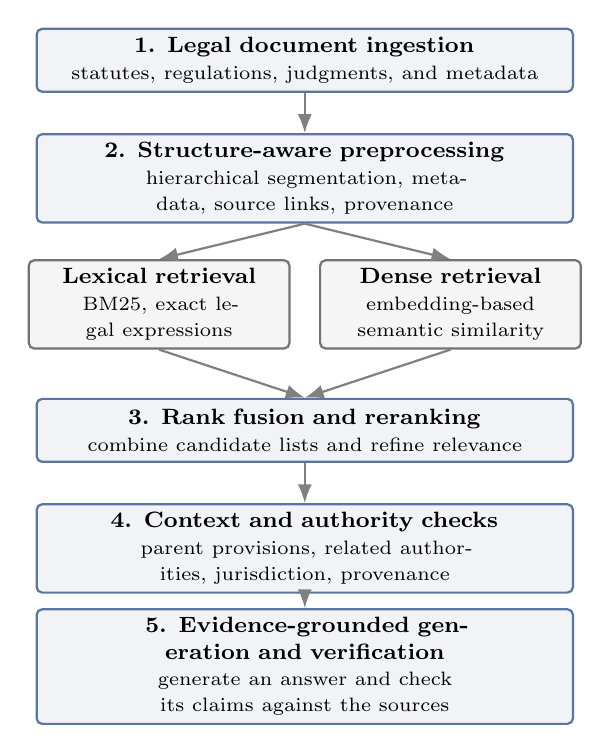
\begin{tikzpicture}[
  font=\footnotesize,
  stage/.style={draw, thick, rounded corners=2pt, align=center, text width=6.6cm,
                minimum height=8mm, inner sep=3pt, fill=legalblue!6, draw=legalblue!70},
  sub/.style={draw, thick, rounded corners=2pt, align=center, text width=3.1cm,
              minimum height=8mm, inner sep=3pt, fill=black!4, draw=black!55},
  fl/.style={-{Latex[length=2.4mm]}, draw=black!50, line width=0.8pt}]

  \node[stage] (ing) at (0,0) {\textbf{1. Legal document ingestion}\\\scriptsize statutes, regulations, judgments, and metadata};
  \node[stage] (pre) at (0,-1.5) {\textbf{2. Structure-aware preprocessing}\\\scriptsize hierarchical segmentation, metadata, source links, provenance};
  \node[sub] (lex) at (-1.85,-3.1) {\textbf{Lexical retrieval}\\\scriptsize BM25, exact legal expressions};
  \node[sub] (den) at ( 1.85,-3.1) {\textbf{Dense retrieval}\\\scriptsize embedding-based semantic similarity};
  \node[stage] (fus) at (0,-4.7) {\textbf{3. Rank fusion and reranking}\\\scriptsize combine candidate lists and refine relevance};
  \node[stage] (ctx) at (0,-6.2) {\textbf{4. Context and authority checks}\\\scriptsize parent provisions, related authorities, jurisdiction, provenance};
  \node[stage] (gen) at (0,-7.7) {\textbf{5. Evidence-grounded generation and verification}\\\scriptsize generate an answer and check its claims against the sources};

  \draw[fl] (ing) -- (pre);
  \draw[fl] (pre.south) -- (lex.north);
  \draw[fl] (pre.south) -- (den.north);
  \draw[fl] (lex.south) -- (fus.north);
  \draw[fl] (den.south) -- (fus.north);
  \draw[fl] (fus) -- (ctx);
  \draw[fl] (ctx) -- (gen);
\end{tikzpicture}}
\caption{Conceptual architecture synthesizing complementary legal retrieval methods. This is a
proposed reference architecture, not a claim that every component has been validated together in a
single experiment.}
\label{fig:arch}
\end{figure}


A knowledge graph can be connected to the context-and-authority stage to discover relationships among
retrieved sources. An agentic controller may also invoke retrieval again when the evidence is
incomplete or contradictory. Both additions should be justified by measurable benefits rather than
included merely to increase architectural complexity.

\subsection{How retrieval architectures should be evaluated}

A retrieval architecture should be assessed independently from the quality of its generated answers.
If the retrieval component does not return the required evidence, the generator's output cannot
reliably compensate for that failure. Conversely, successful retrieval does not establish that the
generator will interpret the evidence correctly. Several complementary metrics are useful, as
summarized in Table~\ref{tab:metrics}.

\begin{table*}[tp]
\centering
\caption{Complementary metrics for evaluating legal retrieval architectures.}
\label{tab:metrics}
\footnotesize
\setlength{\tabcolsep}{5pt}
\renewcommand{\arraystretch}{1.3}
\begin{tabularx}{\textwidth}{>{\raggedright\arraybackslash}p{4.2cm} >{\raggedright\arraybackslash}X >{\raggedright\arraybackslash}X}
\toprule
\textbf{Metric} & \textbf{What it measures} & \textbf{Why it matters in legal retrieval} \\
\midrule
Recall@$k$ & Whether relevant evidence appears among the top $k$ retrieved results. & Measures the system's ability to find needed authorities or passages. \\
Precision@$k$ & The proportion of the top $k$ results that are relevant. & Indicates how much irrelevant material may enter the generation context. \\
Mean Reciprocal Rank (MRR) & The reciprocal rank of the first relevant result, averaged across queries. & Measures how early the system finds a relevant passage. \\
Normalized Discounted Cumulative Gain (nDCG) & Ranking quality when results have graded relevance. & Helps distinguish highly relevant legal evidence from merely related passages. \\
Citation precision & The proportion of supplied citations that correctly support their associated claims, under a defined annotation protocol. & Measures whether references are actually evidentially useful. \\
Citation recall & The proportion of required supporting sources or claims that receive appropriate citations, under a defined protocol. & Helps detect missing legal support. \\
Unsupported-claim rate & The proportion of evaluated claims that lack adequate support in the permitted evidence. & Evaluates grounding beyond the presence of citations. \\
Latency and cost & Time and computational or service cost per query. & Helps determine whether architectural improvements are practical. \\
\bottomrule
\end{tabularx}
\end{table*}

These metrics require clear annotation guidelines. For example, relevance may be graded at the document
level or the passage level; the two can produce different results. Similarly, citation correctness
requires an explicit definition of what counts as support. A citation that mentions the same topic is
not necessarily a citation that substantiates the claim.

A rigorous evaluation should therefore use a consistent query set and legal corpus, compare lexical,
dense, hybrid, and structure-aware configurations under controlled conditions, and measure both
retrieval and final answer reliability. Where feasible, ablation studies should remove one component at
a time to determine whether improvements can be attributed to rank fusion, structural metadata,
reranking, graph traversal, or another architectural choice.

\subsection{Synthesis and remaining research challenges}

The development of legal retrieval architectures reflects a progression from finding text that matches
a query toward identifying evidence that is relevant, structurally contextualized, and suitable for
supporting a legal conclusion. Lexical retrieval provides a strong foundation for exact legal
terminology. Dense retrieval addresses differences in wording. Hybrid retrieval and rank fusion combine
complementary signals, while reranking refines the candidate set. Structure-aware indexing preserves
the organization of legal documents, and knowledge graphs can connect authorities across documents.

None of these components independently guarantees legal correctness. Their value depends on the legal
corpus, source provenance, retrieval configuration, quality of metadata, and evaluation protocol. A
sophisticated retriever can still return an incomplete set of authorities, while a well-ranked passage
can remain insufficient if its parent provision or relevant exception is missing.

The resulting research direction is not simply to build a larger or more complicated retrieval
pipeline. It is to design systems in which the evidence required for a legal answer can be retrieved,
contextualized, and verified systematically. This provides the technical foundation for the next part
of the survey, which examines hallucination, factual support, and citation correctness as separate but
connected dimensions of legal AI reliability.

\section{Reliability, Hallucination, and Legal Citation Verification}
\label{sec:reliability}

\subsection{From relevant retrieval to reliable legal answers}

Retrieval-augmented generation (RAG) has become an important approach to reducing the dependence of
large language models (LLMs) on parametric knowledge alone. By retrieving external documents at
inference time, a RAG system can provide answers grounded in legal statutes, regulations, judgments,
and other authoritative materials. However, access to external evidence does not automatically make an
answer reliable. A system may retrieve a relevant document but misinterpret its legal meaning, overlook
an exception, cite the wrong passage, or generate a conclusion that the retrieved evidence does not
support.

This distinction is particularly important in law because legal correctness depends on more than
textual similarity. An answer may accurately reproduce a sentence from a judgment while misrepresenting
its holding. It may identify the correct statute but overlook an amendment, jurisdictional restriction,
procedural condition, or subsequent decision that affects its application. Consequently, reliability
must be evaluated across the complete pipeline, from evidence retrieval to legal interpretation and
citation generation.

The reliability problem can be understood through three related questions:
\begin{enumerate}[leftmargin=1.4em, itemsep=2pt, topsep=2pt]
\item \textbf{Was the right evidence retrieved?} The system must locate the relevant legal provision,
passage, or judgment.
\item \textbf{Does the evidence support the claim?} The generated statement must follow from the cited
material rather than merely discuss a similar topic.
\item \textbf{Is the claim legally applicable?} The system must account for relevant jurisdiction,
temporal validity, procedural context, and legal authority.
\end{enumerate}

These questions are related but not interchangeable. A system can perform well on retrieval metrics and
still generate unsupported conclusions. Similarly, a response containing accurate quotations may remain
misleading if it applies them to the wrong legal issue.

\subsection{Types of reliability failures}

Legal AI reliability is not a single measurable property. It includes several failure modes that
require different detection and mitigation strategies, as summarized in Table~\ref{tab:failures}.

\begin{table*}[tp]
\centering
\caption{Reliability failure modes in legal AI and possible mitigations.}
\label{tab:failures}
\footnotesize
\setlength{\tabcolsep}{5pt}
\renewcommand{\arraystretch}{1.3}
\begin{tabularx}{\textwidth}{>{\raggedright\arraybackslash}p{2.5cm} >{\raggedright\arraybackslash}X >{\raggedright\arraybackslash}X >{\raggedright\arraybackslash}X}
\toprule
\textbf{Failure type} & \textbf{Description} & \textbf{Illustrative example} & \textbf{Possible mitigation} \\
\midrule
Fabricated authority & The system invents a case, statute, provision, or citation. & Referring to a nonexistent judgment. & Citation resolution against authoritative databases. \\
Incorrect citation & A real source is cited, but the cited passage does not support the associated claim. & Citing a procedural provision as authority for a substantive conclusion. & Claim-to-passage entailment checking. \\
Unsupported claim & The response makes a factual or legal assertion that is not established by retrieved evidence. & Stating that a remedy is available without retrieving the relevant conditions. & Evidence coverage checks and abstention. \\
Misinterpretation & The source is real, but its legal meaning is misrepresented. & Treating an observation as the court's binding holding. & Role-aware judgment analysis and contextual verification. \\
Incomplete evidence & A relevant exception, counter-authority, or condition is omitted. & Explaining a general rule without its statutory exception. & Query expansion and retrieval of related provisions. \\
Outdated law & The system relies on a superseded or inapplicable version of a legal source. & Applying an earlier statutory amendment. & Effective-date metadata and version-aware retrieval. \\
Jurisdictional mismatch & The system applies law from a different jurisdiction. & Using an Indian legal rule to answer a Pakistani-law question. & Jurisdiction filtering and authority classification. \\
Contradictory evidence & The system fails to reconcile conflicting authorities. & Presenting one judgment without acknowledging a relevant later ruling. & Authority-aware ranking and explicit conflict reporting. \\
\bottomrule
\end{tabularx}
\end{table*}

The categories overlap. For example, a jurisdictional mismatch may also produce an unsupported claim,
while outdated law can lead to incorrect citations. Nevertheless, distinguishing the underlying failure
is useful because a single safeguard cannot address every problem.

\subsection{Evidence grounding and citation correctness}

A citation should not be treated as reliable merely because it points to an existing document. Legal
citation verification requires checking both the existence of the source and its relationship to the
claim. A practical verification process separates four operations:
\begin{itemize}[leftmargin=1.4em, itemsep=2pt, topsep=2pt]
\item \textbf{Citation resolution:} Determine whether the cited statute, case, section, paragraph, or
other authority exists and can be located.
\item \textbf{Passage verification:} Confirm that the cited passage contains the relevant legal
language or reasoning.
\item \textbf{Claim-support verification:} Assess whether the passage actually supports the claim,
rather than simply sharing vocabulary with it.
\item \textbf{Applicability verification:} Check whether the authority is relevant to the jurisdiction,
date, issue, and procedural context of the question.
\end{itemize}

This process suggests that citation verification should operate at the level of individual claims, not
merely at the level of the complete response. A long answer may contain several supported statements and
one critical unsupported conclusion. Evaluating the answer as a single unit can obscure that distinction.

LegalBench-RAG addresses an important part of this problem by focusing on retrieving precise legal text
segments rather than relying solely on document-level retrieval. Its benchmark design reinforces the
importance of locating evidence at a sufficiently granular level for downstream legal tasks
\citep{pipitone2024}. However, precise retrieval and legal entailment remain separate requirements:
finding the correct passage does not itself establish that the generated interpretation is valid.

\citet{dahl2024}, in their discussion of fabricated legal authorities and the broader reliability of
generative AI in law, and \citet{magesh2025}, in their assessment of leading AI legal research tools,
further motivate evaluating the output rather than assuming that fluent language or a citation list
indicates correctness. These studies should not be interpreted as establishing one universal
hallucination rate for all legal AI systems. Results depend on the tools, tasks, jurisdictions, test
sets, and definitions of error used in each evaluation.

\subsection{Evaluating reliability: beyond answer accuracy}

A robust evaluation framework should distinguish retrieval quality, citation quality, factual or legal
support, and operational performance. No single metric captures all of these dimensions, as
Table~\ref{tab:releval} shows.

\begin{table*}[tp]
\centering
\caption{Dimensions for evaluating legal AI reliability.}
\label{tab:releval}
\footnotesize
\setlength{\tabcolsep}{5pt}
\renewcommand{\arraystretch}{1.3}
\begin{tabularx}{\textwidth}{>{\raggedright\arraybackslash}p{2.6cm} >{\raggedright\arraybackslash}p{2.9cm} >{\raggedright\arraybackslash}X >{\raggedright\arraybackslash}X}
\toprule
\textbf{Evaluation dimension} & \textbf{Example metric} & \textbf{What it measures} & \textbf{Important limitation} \\
\midrule
Retrieval effectiveness & Recall@$k$ & Whether relevant evidence appears among the top $k$ retrieved results. & Does not measure whether the final answer uses that evidence correctly. \\
Ranking quality & MRR or nDCG & How effectively the system ranks relevant passages. & Depends on relevance judgments and benchmark design. \\
Citation validity & Citation validity rate & Proportion of generated citations that resolve to real sources. & A real citation may still be irrelevant or misleading. \\
Citation support & Claim--citation support rate & Proportion of claims adequately supported by their cited evidence. & Requires careful annotation or reliable support verification. \\
Evidence coverage & Evidence coverage rate & Extent to which material claims have supporting evidence. & Does not establish that the evidence is legally correct or complete. \\
Unsupported content & Unsupported-claim rate & Proportion of claims lacking adequate evidential support. & Results vary with claim segmentation and annotation policy. \\
Legal correctness & Expert-assessed correctness & Whether the answer's legal analysis is judged correct under the task conditions. & Requires qualified evaluators and explicit jurisdictional criteria. \\
Calibration & Confidence--accuracy alignment & Whether confidence corresponds to observed correctness. & Model-reported confidence can be poorly calibrated. \\
Efficiency & Latency and cost per query & Operational expense of producing an answer. & Low cost or latency does not imply legal reliability. \\
\bottomrule
\end{tabularx}
\end{table*}

Metric definitions should be fixed before evaluation. For example, citation validity rate and citation
support rate should not be used interchangeably. A citation can be valid in the first sense and invalid
in the second. Likewise, an unsupported-claim rate should specify whether the denominator consists of
all generated claims, all material claims, or all claims requiring citations.

Evaluation should also distinguish automatic checks from expert assessment. Automated tools can identify
broken links, malformed citations, missing sources, and some forms of semantic inconsistency. Human
legal reviewers remain important for assessing nuanced statutory interpretation, the relative authority
of cases, exceptions, and whether a response appropriately qualifies uncertainty. Ideally, evaluations
should report the annotation protocol, reviewer expertise, agreement between reviewers, and adjudication
procedure.

\subsection{Safeguards for legal AI applications}

Reliability is best addressed through multiple safeguards rather than a single verification component:
\begin{enumerate}[leftmargin=1.4em, itemsep=2pt, topsep=2pt]
\item \textbf{Authoritative source management.} Record provenance, jurisdiction, document identity,
effective dates, and amendments.
\item \textbf{Evidence retrieval and ranking.} Retrieve relevant passages using lexical, dense, hybrid,
or structure-aware methods.
\item \textbf{Claim-level generation.} Associate material legal claims with specific supporting
passages.
\item \textbf{Verification and conflict checks.} Resolve citations, test claim support, and identify
missing or conflicting authorities.
\item \textbf{Qualified response or abstention.} Answer with traceable evidence, state uncertainty, or
decline to make an unsupported conclusion.
\end{enumerate}
\textit{This is a conceptual reliability workflow synthesized for this survey; it is not a claim that
every reviewed system implements all five stages.}

The workflow highlights several design principles. First, provenance and temporal metadata should be
preserved during ingestion rather than added after generation. Second, verification should be applied
to material claims and their supporting passages. Third, the system should be allowed to abstain when
evidence is missing or contradictory. Finally, high-impact legal applications should preserve access to
the underlying sources and support review by a qualified human.

Agentic architectures can coordinate these safeguards through retrieval, verification, and revision
steps. However, adding more agents does not automatically improve correctness. If the agents rely on the
same incomplete corpus or repeat the same unsupported assumption, orchestration may reproduce rather
than correct the error. Reliability therefore depends on independent evidence checks, explicit
verification criteria, and measurable performance improvements.

\subsection{Section synthesis}

The central lesson is that legal AI reliability must be evaluated as an evidence-to-claim problem.
Retrieval quality is necessary, but it is not sufficient. A dependable system must retrieve appropriate
authority, preserve its context, generate claims that follow from the evidence, verify citations, and
recognize when legal applicability remains uncertain. These requirements motivate the comparative
analysis in the next section, where contemporary systems are assessed according to their evidence
sources, retrieval design, legal reasoning, verification mechanisms, and evaluation practices.

\subsection{Implications for evaluation and reproducibility}

The literature also highlights a methodological problem: reliability results cannot be compared fairly
unless the underlying evaluation conditions are reported. A hallucination rate obtained from open-ended
questions about legal doctrine is not directly comparable with one obtained from citation verification,
statutory question answering, or retrieval of annotated passages.

For example, \citet{magesh2025} evaluated commercial legal research tools and found that hallucinations
persisted despite the use of RAG. Their findings challenge claims that retrieval alone can guarantee
hallucination-free outputs. \citet{dahl2024} likewise documented substantial hallucination problems in
general-purpose LLMs answering legal questions. A reproducible legal AI evaluation should therefore
disclose:
\begin{itemize}[leftmargin=1.4em, itemsep=2pt, topsep=2pt]
\item the jurisdiction, legal domain, and temporal scope of the corpus;
\item the source of questions and the criteria used to construct the test set;
\item the operational definition of hallucination and unsupported claims;
\item the annotation instructions, reviewer expertise, and agreement statistics;
\item the retrieval configuration, model version, prompts, and verification settings;
\item the baseline systems, uncertainty estimates, and statistical tests where appropriate.
\end{itemize}

These requirements are especially important when evaluating improvements from hybrid retrieval,
reranking, knowledge graphs, or agentic verification. Each component should be assessed through
controlled comparisons or ablation studies, rather than attributing all observed improvements to the
complete architecture.

The resulting research priority is clear: legal AI needs not only more capable models, but also
transparent evidence pipelines and evaluations that measure whether answers are actually supported by
applicable legal authority.

\section{Comparative Analysis of Contemporary Legal AI Systems}
\label{sec:comparison}

\subsection{A common framework for comparing legal AI architectures}

Contemporary legal AI systems differ not only in the models they use but also in how they retrieve,
organize, interpret, and verify legal evidence. A fair comparison must therefore examine the complete
processing pipeline rather than focusing exclusively on the underlying language model or a reported
accuracy score. This section compares representative systems using six dimensions:
\begin{enumerate}[leftmargin=1.4em, itemsep=2pt, topsep=2pt]
\item \textbf{Architecture:} how the system organizes its processing components.
\item \textbf{Retrieval strategy:} how it identifies and ranks relevant legal material.
\item \textbf{Generation method:} how it produces classifications, legal analysis, or drafted text.
\item \textbf{Evidence verification:} whether it checks source validity and claim-level support.
\item \textbf{Evaluation:} how its performance is measured.
\item \textbf{Limitations:} what its architecture or experimental design does not establish.
\end{enumerate}

The comparison distinguishes between legal language models, benchmarks, retrieval systems, and
end-to-end applications. This distinction is necessary because a benchmark such as LegalBench-RAG
evaluates a specific capability, whereas a platform such as JusBuild is designed to support a legal
workflow. Their contributions are complementary, but they cannot be ranked directly without common
experiments. A benchmark for legal classification cannot establish that a system is reliable at
retrieving current statutes, and a document-drafting system cannot automatically be considered
superior to a legal search system.

\subsection{Architecture and retrieval strategy}

Table~\ref{tab:arch8} compares the architecture and retrieval strategy of representative legal AI
approaches.

\begin{table*}[tp]
\centering
\caption{Architectural comparison of representative legal AI approaches.}
\label{tab:arch8}
\footnotesize
\setlength{\tabcolsep}{5pt}
\renewcommand{\arraystretch}{1.3}
\begin{tabularx}{\textwidth}{>{\raggedright\arraybackslash}p{2.8cm} >{\raggedright\arraybackslash}X >{\raggedright\arraybackslash}X >{\raggedright\arraybackslash}X}
\toprule
\textbf{System} & \textbf{Architecture} & \textbf{Retrieval strategy} & \textbf{Generation or output method} \\
\midrule
LEGAL-BERT \citep{chalkidis2020} & Legal-domain pretrained transformer & Not inherently a retrieval system & Contextual representations for downstream legal NLP tasks \\
LexGLUE \citep{chalkidis2022} & Benchmark suite for legal language understanding & Depends on the evaluated model and task & Task-specific predictions, such as classification \\
LegalBench \citep{guha2023} & Multi-task legal reasoning benchmark & Not a single retrieval architecture & Model-generated answers or task outputs evaluated against task-specific criteria \\
LegalBench-RAG \citep{pipitone2024} & Retrieval benchmark with annotated legal text segments & Evaluates retrieval of relevant legal passages & Evaluates retrieval rather than prescribing one answer-generation architecture \\
JusBuild \citep{buffa2025} & Structured legal document-building workflow & Document segmentation and vector-based retrieval & Combines retrieved precedent material with AI-assisted drafting and human oversight \\
Pakistani legal RAG framework \citep{ref312025} & Jurisdiction-specific question-answering pipeline & Hybrid keyword and semantic retrieval & LLM-generated legal answers grounded in retrieved materials \\
Ren et al.\ \citep{ren2026} & Legal LLM improvement pipeline incorporating data synthesis and RAG & Retrieval-augmented generation alongside synthetic-data development & Legal LLM outputs assessed through benchmark and model-evaluation procedures \\
Legalyze \citep{hamza2026} & Structure-aware, agentic legal RAG platform & Hierarchical indexing, lexical and dense retrieval, reciprocal-rank fusion & Agentic legal analysis and synthesis grounded in retrieved legal evidence \\
\bottomrule
\end{tabularx}
\end{table*}

The table demonstrates that architectural differences correspond to different research objectives.
Domain-adapted transformers aim to improve the model's understanding of legal language. Retrieval
benchmarks measure whether relevant evidence can be found. End-to-end RAG applications combine
retrieval with generation, while structure-aware systems additionally attempt to preserve
relationships within legal documents.

These differences matter because a model that performs well on a legal classification task may not
retrieve the relevant statutory provision, and a system that retrieves the right passage may still
misinterpret its legal meaning. The architecture must therefore be assessed against the particular
failure modes it is intended to address.

\subsection{Evidence verification and evaluation}

Table~\ref{tab:evid8} summarizes evidence handling and evaluation considerations across the same
systems.

\begin{table*}[tp]
\centering
\caption{Evidence handling and evaluation considerations.}
\label{tab:evid8}
\footnotesize
\setlength{\tabcolsep}{5pt}
\renewcommand{\arraystretch}{1.3}
\begin{tabularx}{\textwidth}{>{\raggedright\arraybackslash}p{2.8cm} >{\raggedright\arraybackslash}X >{\raggedright\arraybackslash}X >{\raggedright\arraybackslash}X}
\toprule
\textbf{System or approach} & \textbf{Evidence verification} & \textbf{Evaluation focus} & \textbf{Key limitation to consider} \\
\midrule
LEGAL-BERT & No inherent citation-verification mechanism & Performance on downstream legal NLP tasks & Legal language competence does not establish evidence-grounded reasoning \\
LexGLUE & Determined by the evaluated task and model & Standardized legal language understanding & Task scores do not directly measure citation support \\
LegalBench & Task-dependent; not a universal citation verifier & A broad range of legal reasoning tasks & Performance may vary considerably by task and legal concept \\
LegalBench-RAG & Evaluates retrieval against annotated relevant passages & Passage-level retrieval quality & Does not, by itself, establish the correctness of a generated legal answer \\
JusBuild & Uses a structured drafting workflow with human oversight & Legal document-building performance in its evaluated settings & Human review and drafting performance do not establish general-purpose legal reliability \\
Pakistani legal RAG framework & Evidence is retrieved for grounded answering; verification should be assessed separately & Legal question answering over selected Pakistani legal materials & Grounding alone does not establish source completeness, temporal validity, or claim-level entailment \\
Ren et al. & Retrieval and evaluation components support the broader legal LLM pipeline & Legal model performance and evaluation of generated outputs & Results depend on the selected benchmarks and experimental settings \\
Legalyze & Citation-grounded response design and a hybrid retrieval pipeline & Retrieval and answer reliability within its reported evaluation setting & Performance on one corpus and query set cannot establish universal legal correctness \\
\bottomrule
\end{tabularx}
\end{table*}

A critical distinction emerges: citation presence, citation validity, and citation support are three
different properties. A system may generate a citation, point to an existing legal source, and still
misrepresent what that source establishes. Accordingly, evaluation should measure whether citations
resolve correctly and whether the cited passages support individual claims.

The same caution applies to numerical results. Retrieval recall, legal answer accuracy,
unsupported-claim rate, and citation precision measure different properties. Scores reported on
different datasets or under different annotation protocols should not be compared as if they were
measurements of the same outcome. For this reason, contemporary systems should ideally be evaluated
through a common protocol combining passage-level retrieval metrics, expert-assessed legal
correctness, citation-support analysis, temporal and jurisdictional checks, and operational measures
such as latency and cost.

\subsection{Comparing system design philosophies}

The systems above illustrate three broad design philosophies.

\subsubsection{Model-centric legal AI}

Model-centric approaches improve legal performance by adapting language models to legal text, tasks, or
reasoning patterns. LEGAL-BERT and research evaluated using LexGLUE exemplify this direction. LegalBench
complements it by testing a wider range of legal reasoning capabilities.

The principal advantage is that domain adaptation can improve a model's ability to interpret legal
terminology, identify relevant concepts, and perform specialized NLP tasks. However, model-centric
systems remain limited when a question depends on an authoritative source that was absent from training,
has changed since training, or must be cited precisely.

The key distinction is between understanding legal language and retrieving legally applicable evidence.
A model can recognize the meaning of a statutory provision without establishing whether that provision
is current or whether it applies to the user's specific question.

\subsubsection{Retrieval-centric legal AI}

Retrieval-centric approaches place greater emphasis on locating relevant legal material. LegalBench-RAG
demonstrates the importance of retrieving precise text segments rather than returning only broad
document-level matches. The Pakistani legal RAG framework illustrates the use of hybrid retrieval to
combine semantic similarity with keyword matching.

The main advantage is that answers can be conditioned on external legal sources, reducing dependence on
the model's internal knowledge. Retrieval can also make responses more auditable because a user can
inspect the source passages.

Nevertheless, retrieval quality depends on corpus coverage, document parsing, chunking, query
interpretation, and ranking. Even a highly relevant passage can be misinterpreted or applied outside its
proper legal context. Retrieval-centric systems therefore need a separate mechanism for validating the
relationship between evidence and generated claims.

\subsubsection{Structure-aware and workflow-oriented legal AI}

A third direction combines retrieval with legal document structure, task-specific processing, or
coordinated workflows. JusBuild uses document segmentation and section-level retrieval to assist with
structured drafting. Legalyze combines hierarchical legal indexing with lexical and dense retrieval,
rank fusion, and agentic analysis.

These approaches recognize that legal documents are not simply collections of independent text passages.
A provision belongs to a section, chapter, statute, or legal instrument; a judgment contains procedural
history, arguments, reasoning, and a decision. Preserving this organization can help a system retrieve
the correct passage while retaining the context needed to interpret it.

Workflow-oriented designs can additionally separate retrieval, analysis, synthesis, and verification.
Their potential benefit is improved traceability and more explicit control over intermediate operations.
Their cost is architectural complexity: every additional stage introduces implementation, latency, and
evaluation requirements. The critical question is not whether a system has more components, but whether
those components address identifiable failure modes and produce measurable improvements.

\subsection{Cross-system comparison: capabilities and unresolved gaps}

The comparison can be extended beyond individual systems to the capabilities that a dependable legal AI
platform should support, as set out in Table~\ref{tab:capabilities}.

\begin{table*}[tp]
\centering
\caption{Capabilities of a dependable legal AI platform and associated research directions.}
\label{tab:capabilities}
\footnotesize
\setlength{\tabcolsep}{5pt}
\renewcommand{\arraystretch}{1.3}
\begin{tabularx}{\textwidth}{>{\raggedright\arraybackslash}p{3.0cm} >{\raggedright\arraybackslash}X >{\raggedright\arraybackslash}X >{\raggedright\arraybackslash}X}
\toprule
\textbf{Capability} & \textbf{Why it matters} & \textbf{Typical weakness if omitted} & \textbf{Research direction} \\
\midrule
Legal language understanding & Interprets legal terminology and complex syntax. & Relevant legal meaning may be misunderstood. & Legal-domain adaptation and task-specific evaluation. \\
Hybrid retrieval & Finds both exact legal expressions and semantically related passages. & Statutory identifiers or paraphrased queries may be missed. & Combine lexical and dense retrieval. \\
Rank fusion and reranking & Improves the ordering of candidate evidence. & Relevant passages may remain buried in the result list. & Evaluate fusion and reranking through ablations. \\
Hierarchical indexing & Preserves relationships between passages and their parent documents. & Retrieved fragments may lose statutory or judgment context. & Structure-aware segmentation and metadata. \\
Knowledge-graph retrieval & Represents explicit relations between legal entities and authorities. & Cross-document relationships may remain difficult to retrieve. & Graph construction, entity linking, and graph--text retrieval. \\
Citation verification & Tests whether cited sources exist and support generated claims. & Responses may contain invalid or misleading citations. & Claim-level evidence verification. \\
Temporal and jurisdictional control & Helps ensure that retrieved law is applicable. & Superseded or foreign legal authorities may be used. & Versioned corpora and jurisdiction-aware filtering. \\
Multilingual retrieval & Supports queries expressed in different languages or scripts. & Users may fail to retrieve evidence phrased differently from their query. & Cross-lingual retrieval, transliteration, and legal terminology alignment. \\
Reproducible evaluation & Makes performance claims independently testable. & Improvements may reflect dataset or evaluation differences. & Public test sets, transparent protocols, and statistical analysis. \\
\bottomrule
\end{tabularx}
\end{table*}

This comparison reveals that the main challenge is not necessarily the absence of an individual
technique. Rather, the challenge is integrating these techniques into a coherent pipeline while
preserving evidence provenance and enabling meaningful evaluation. For example, hybrid retrieval and
reranking can improve candidate selection, but neither guarantees that the selected passage is legally
authoritative. Hierarchical indexing can preserve document context, but it does not automatically
establish relationships between separate judgments and statutes. A knowledge graph can encode those
relationships, but its usefulness depends on the accuracy, completeness, and provenance of the graph.
Citation verification can identify unsupported claims, but only if the verification process has access
to suitable evidence and appropriate legal criteria.

\subsection{The Pakistani legal AI context}

The Pakistani legal context provides a useful case study because jurisdiction-specific legal materials
must be interpreted within their own institutional and documentary structures. A system developed
primarily around US or European legal resources cannot be assumed to perform reliably on Pakistani
statutes and judgments without appropriate corpus construction, jurisdictional adaptation, and
evaluation.

\citet{ref312025} describe a RAG-based framework for Pakistani legal question answering that combines
semantic and keyword-based retrieval over selected legal materials, including the Code of Criminal
Procedure and Pakistan Penal Code. This work illustrates the importance of combining legal-domain
evidence with retrieval methods suited to the source material.

Legalyze \citep{hamza2026} follows a related but more structure-aware approach. Its architecture
incorporates hierarchical indexing, lexical and dense retrieval, reciprocal-rank fusion, and agentic
legal analysis over Pakistani legal materials. These design choices address complementary challenges:
lexical retrieval supports exact legal terminology, dense retrieval supports semantic variation, rank
fusion combines result lists, and hierarchical indexing helps preserve legal document organization.

However, a meaningful comparison between the two systems would require a shared evaluation dataset,
consistent query sets, documented corpus coverage, equivalent retrieval budgets, and common measures of
retrieval and answer quality. The existence of hybrid retrieval in both systems is not sufficient to
establish which performs better. Likewise, differences in reported hallucination rates should not be
attributed to a single architectural component unless the experimental design isolates that component.

A further research opportunity concerns multilingual access. Pakistani legal materials and user
questions may involve English, Urdu, and Roman Urdu, while statutory text and case-law terminology may
not map neatly across languages. A robust system must therefore align the user's intended legal concept
with the authoritative terminology used in the source corpus, rather than relying exclusively on literal
translation.

\subsection{A unified framework for comparing legal AI systems}

The preceding analysis suggests that future comparisons should separate four levels of system
performance:
\begin{enumerate}[leftmargin=1.4em, itemsep=3pt, topsep=2pt]
\item \textbf{Retrieval performance.} Does the system find the relevant legal material and rank it
appropriately? \textit{Measures:} Recall@$k$, MRR, nDCG, passage-level precision.
\item \textbf{Evidence integrity.} Does the system preserve source identity, document context, temporal
validity, and jurisdiction? \textit{Measures:} source resolution, provenance completeness, temporal and
jurisdictional error rates.
\item \textbf{Legal answer quality.} Does the answer correctly interpret and apply the retrieved
authority? \textit{Measures:} expert-assessed correctness, claim support, citation accuracy,
unsupported-claim rate.
\item \textbf{Operational performance.} Can the system provide useful results within acceptable
computational and review costs? \textit{Measures:} latency, computational cost, failure recovery, and
human review burden.
\end{enumerate}

This framework discourages the use of one aggregate score to conceal important weaknesses. A system may
retrieve highly relevant passages but generate inaccurate legal conclusions; another may generate
convincing answers but rely on incomplete or outdated evidence. Reporting each level separately makes
such trade-offs visible. Future comparative studies should also report whether the system is
open-source, whether its corpus and evaluation data are accessible, whether its outputs can be
reproduced, and whether its architecture supports independent component replacement.

\subsection{What the comparison reveals}

Three conclusions follow from the comparison. First, no single architectural family addresses every
legal AI problem. Domain-specific language models improve legal language processing, retrieval systems
improve access to external evidence, and structured workflows can coordinate more specialized
operations.

Second, evidence verification remains distinct from evidence retrieval. Lexical retrieval, dense
retrieval, reranking, and rank fusion can improve the candidate evidence presented to a model. They do
not automatically establish that the final answer is supported by that evidence.

Third, jurisdiction and document structure should be treated as architectural requirements rather than
optional metadata. A system that retrieves semantically similar passages without considering the
governing jurisdiction, the document hierarchy, or the effective date of a provision can return
plausible but legally inapplicable evidence. These observations motivate the next section, which
examines jurisdiction-specific reasoning, legal hierarchy, and multilingual access.

\section{Jurisdiction, Document Structure, and Multilingual Legal AI}
\label{sec:jurisdiction}

\subsection{Why legal information retrieval is jurisdiction-dependent}

Legal information retrieval differs from general-purpose information retrieval because the relevance of a
document depends not only on its subject matter but also on its legal authority, jurisdiction, temporal
validity, and relationship to the question being asked. Two passages may discuss the same legal
principle while having different implications because they originate from different jurisdictions or
occupy different positions within a legal system.

For example, a question concerning criminal procedure in Pakistan should prioritize applicable Pakistani
legislation and relevant Pakistani judicial decisions. A semantically similar provision from another
jurisdiction may help explain a general concept, but it should not automatically be treated as governing
authority. Jurisdiction-sensitive retrieval must therefore consider several factors:
\begin{itemize}[leftmargin=1.4em, itemsep=2pt, topsep=2pt]
\item \textbf{Territorial and institutional jurisdiction:} whether the authority applies to the relevant
court, territory, or legal institution.
\item \textbf{Authority type:} whether a document is legislation, a regulation, a binding judgment, a
persuasive judgment, or secondary commentary.
\item \textbf{Temporal validity:} whether the provision or interpretation was applicable at the relevant
time.
\item \textbf{Procedural context:} whether the authority addresses the procedural stage and legal issue
involved.
\item \textbf{Precedential relationships:} whether a judgment follows, distinguishes, overrules, or
otherwise relates to another decision.
\end{itemize}

These considerations expose a limitation of conventional semantic retrieval. An embedding model may
identify two passages as highly similar without determining whether either passage is legally
applicable. Consequently, jurisdictional and temporal constraints should influence retrieval and
verification, not merely appear as explanatory text in the final answer.

\subsection{Legal hierarchy and document structure}

Legal documents contain multiple layers of organization. Statutes may be divided into parts, chapters,
sections, subsections, clauses, and provisos. Judgments may contain procedural histories, questions of
law, arguments, judicial reasoning, and final orders. These structural elements help determine the
meaning and applicability of individual passages.

A conventional chunking strategy often divides documents into fixed-size text segments or overlapping
windows. Although computationally convenient, this can separate a provision from its heading, definition,
exception, proviso, or parent section. The resulting fragment may remain semantically understandable
while losing context that is essential to legal interpretation. Consider a hypothetical example:

\begin{quote}
\textit{Illustrative statutory structure (schematic):}
\begin{itemize}[leftmargin=1.3em, itemsep=1pt, topsep=2pt]
\item \textbf{Chapter III: General Conditions}
  \begin{itemize}[leftmargin=1.2em, itemsep=1pt, topsep=1pt]
  \item \textbf{Section 12 (general rule):} a person may exercise the stated right subject to the
  conditions specified in this section.
    \begin{itemize}[leftmargin=1.2em, itemsep=1pt, topsep=1pt]
    \item \textbf{Subsection (2) (limitation):} the right is subject to the additional restrictions
    specified in the subsection.
    \item \textbf{Proviso:} an exception applies where the specified conditions are satisfied.
    \end{itemize}
  \end{itemize}
\end{itemize}
This is an illustrative structure only, not an actual statutory provision.
\end{quote}

If retrieval returns only the general rule, the generated answer may omit the limitation or exception.
If it returns only the proviso, the system may fail to explain the general rule to which that exception
applies. Structure-aware retrieval addresses this problem by preserving the relationship between a
passage and its parent document elements. Useful techniques include:
\begin{enumerate}[leftmargin=1.4em, itemsep=2pt, topsep=2pt]
\item \textbf{Hierarchical metadata:} storing the document, chapter, section, subsection, and paragraph
identifiers associated with each passage.
\item \textbf{Context-preserving chunking:} retaining headings, definitions, exceptions, and relevant
neighboring passages.
\item \textbf{Parent-child retrieval:} retrieving a focused passage while allowing the system to recover
its broader context.
\item \textbf{Reference resolution:} linking references to other sections, definitions, schedules, and
related legal instruments.
\item \textbf{Provenance preservation:} maintaining the source document, version, location, and other
information needed to verify the passage.
\end{enumerate}

Structure-aware indexing and knowledge-graph retrieval are complementary. Hierarchical indexing preserves
the organization of a document, whereas a knowledge graph represents explicit relationships between
entities, legal provisions, judgments, and other objects. A system may use both, but each requires
separate construction and evaluation.

\subsection{Pakistani legal information retrieval}

Pakistan provides a useful case study of the challenges involved in building jurisdiction-aware legal
AI. Its legal information needs span constitutional provisions, statutes, procedural codes, judicial
decisions, and other legal materials. A useful system must preserve the relationships among these
sources rather than treating every retrieved passage as an interchangeable text fragment.

For example, the Constitution of Pakistan, the Pakistan Penal Code (PPC), the Code of Criminal Procedure
(CrPC), the Qanun-e-Shahadat Order (QSO), and judicial decisions serve different legal functions. The
appropriate source depends on the question. A constitutional question may require a constitutional
provision and relevant case law, while a question about a criminal procedure may require the applicable
procedural provision and related judicial interpretation.

Three challenges are particularly important. First, \textit{document coverage and authority.} A corpus
may contain a large volume of legal text but still omit relevant amendments, judgments, or authoritative
documents. Corpus size alone is therefore an inadequate measure of legal coverage. Second, \textit{legal
relationships.} A statutory provision may depend on a definition elsewhere in the same enactment or be
interpreted by a later judgment. Retrieval should preserve these relationships where relevant, rather
than relying exclusively on textual similarity. Third, \textit{temporal and jurisdictional
applicability.} A provision's wording, legal status, or interpretation may change over time. Systems
should record source dates and applicable versions, and distinguish the date of a judgment from the
period in which the underlying law applied.

A jurisdiction-aware Pakistani legal retrieval system should consequently combine source provenance,
hierarchical indexing, authority-aware ranking, and temporal metadata. These features can improve the
reliability of evidence selection, although they do not eliminate the need for legal interpretation and
claim-level verification.

\subsection{English, Urdu, and low-resource legal retrieval}

Multilingual legal AI introduces an additional challenge: the language of a user's query may differ from
the language, terminology, or script of the authoritative source. This is particularly relevant when
users express legal questions in Urdu or Roman Urdu while the source material they need is written in
English.

A multilingual system must bridge differences in vocabulary, spelling, transliteration, morphology, and
legal terminology. Direct translation alone may be insufficient because legal concepts can have
jurisdiction-specific meanings that do not map exactly across languages. Four technical approaches are
particularly relevant, as summarized in Table~\ref{tab:multilingual}.

\begin{table*}[tp]
\centering
\caption{Technical approaches to multilingual legal retrieval.}
\label{tab:multilingual}
\footnotesize
\setlength{\tabcolsep}{5pt}
\renewcommand{\arraystretch}{1.3}
\begin{tabularx}{\textwidth}{>{\raggedright\arraybackslash}p{3.2cm} >{\raggedright\arraybackslash}X >{\raggedright\arraybackslash}X >{\raggedright\arraybackslash}X}
\toprule
\textbf{Approach} & \textbf{How it works} & \textbf{Main advantage} & \textbf{Main limitation} \\
\midrule
Query translation & Translates the query into the language of the source corpus. & Enables use of existing monolingual retrieval infrastructure. & Translation may distort legal terms or procedural meaning. \\
Multilingual dense retrieval & Maps queries and documents from different languages into a shared embedding space. & Supports cross-language semantic matching. & Similar embeddings do not guarantee legal-concept equivalence. \\
Transliteration normalization & Normalizes alternative representations of words across scripts. & Helps retrieve Roman Urdu and Urdu variants. & Many transliterations are ambiguous or inconsistent. \\
Legal terminology alignment & Links expressions to jurisdiction-specific legal concepts and authoritative terms. & Improves conceptual consistency. & Requires curated terminology, entity linking, or legal-domain resources. \\
\bottomrule
\end{tabularx}
\end{table*}

A practical architecture can combine these methods rather than relying on one. Language identification
and transliteration normalization can first process the query. Legal entity linking and terminology
alignment can then identify important statutes, provisions, courts, or legal concepts. Retrieval can
search both the original query and its normalized or translated variants, followed by rank fusion and
legal-context filtering.

The system should preserve the original user query and the original authoritative passage. Translation
can support retrieval, but the final answer should not silently substitute a translated interpretation
for the governing source text.

Evaluation should also be multilingual. An English-only benchmark cannot establish whether the system
works reliably for Urdu or Roman Urdu. Separate evaluation should measure retrieval recall, citation
support, legal correctness, and robustness to spelling and transliteration variation across each
supported query language.

\subsection{Integrating jurisdiction, hierarchy, and multilingual processing}

The three challenges discussed above are interdependent. Language normalization may help locate a
relevant provision, but document structure is needed to preserve its context. Hierarchical indexing may
identify the correct section, but jurisdictional and temporal checks are still required to determine its
applicability. A conceptual architecture connecting these stages is shown in Figure~\ref{fig:mlarch}.

% Conceptual architecture: multilingual, jurisdiction- and structure-aware legal retrieval. Vector TikZ.
\begin{figure}[t]
\centering
\resizebox{\columnwidth}{!}{%
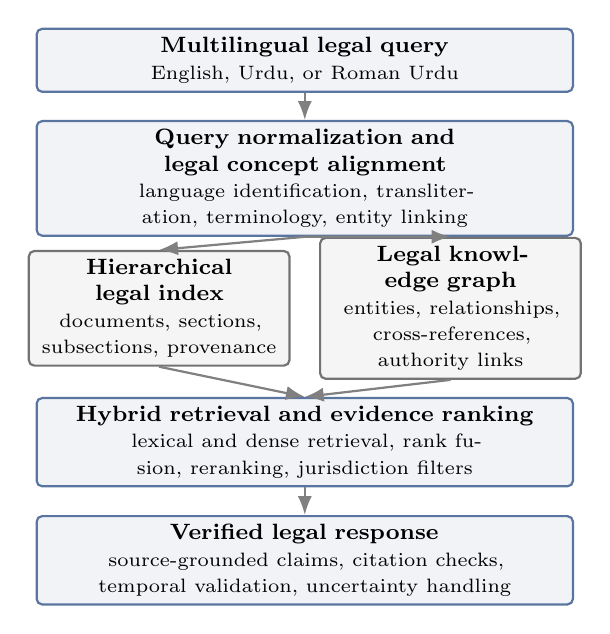
\begin{tikzpicture}[
  font=\footnotesize,
  stage/.style={draw, thick, rounded corners=2pt, align=center, text width=6.6cm,
                minimum height=8mm, inner sep=3pt, fill=legalblue!6, draw=legalblue!70},
  sub/.style={draw, thick, rounded corners=2pt, align=center, text width=3.1cm,
              minimum height=8mm, inner sep=3pt, fill=black!4, draw=black!55},
  fl/.style={-{Latex[length=2.4mm]}, draw=black!50, line width=0.8pt}]

  \node[stage] (q) at (0,0) {\textbf{Multilingual legal query}\\\scriptsize English, Urdu, or Roman Urdu};
  \node[stage] (norm) at (0,-1.5) {\textbf{Query normalization and legal concept alignment}\\\scriptsize language identification, transliteration, terminology, entity linking};
  \node[sub] (idx) at (-1.85,-3.15) {\textbf{Hierarchical legal index}\\\scriptsize documents, sections, subsections, provenance};
  \node[sub] (kg) at ( 1.85,-3.15) {\textbf{Legal knowledge graph}\\\scriptsize entities, relationships, cross-references, authority links};
  \node[stage] (ret) at (0,-4.85) {\textbf{Hybrid retrieval and evidence ranking}\\\scriptsize lexical and dense retrieval, rank fusion, reranking, jurisdiction filters};
  \node[stage] (resp) at (0,-6.35) {\textbf{Verified legal response}\\\scriptsize source-grounded claims, citation checks, temporal validation, uncertainty handling};

  \draw[fl] (q) -- (norm);
  \draw[fl] (norm.south) -- (idx.north);
  \draw[fl] (norm.south) -- (kg.north);
  \draw[fl] (idx.south) -- (ret.north);
  \draw[fl] (kg.south) -- (ret.north);
  \draw[fl] (ret) -- (resp);
\end{tikzpicture}}
\caption{Conceptual architecture connecting multilingual query understanding, legal document structure,
knowledge graphs, retrieval, and evidence verification. Synthesized for this survey; its individual
components require empirical evaluation before any performance improvement can be claimed.}
\label{fig:mlarch}
\end{figure}


This architecture offers a research framework for connecting multilingual query understanding, legal
document structure, knowledge graphs, retrieval, and evidence verification. It also provides a basis for
modular implementation: individual components can be replaced or evaluated independently without
redesigning the entire platform.

\subsection{Section synthesis}

Jurisdiction, document structure, and language are not peripheral concerns in legal information
retrieval. They determine which evidence should be retrieved, how its meaning should be interpreted, and
whether it applies to the question being asked.

For Pakistani legal AI, the main implication is that effective retrieval requires more than semantic
similarity. Systems should preserve legal hierarchy, authority relationships, temporal metadata, source
provenance, and cross-language concept alignment. These requirements lead directly to the open
challenges discussed next.

\section{Open Challenges and Future Research Directions}
\label{sec:future}

\subsection{From capable legal AI to dependable legal information retrieval}

The preceding sections show that contemporary legal AI has made progress in legal language
understanding, evidence retrieval, document drafting, and agentic processing. However, these
capabilities remain difficult to integrate into a system that consistently returns relevant, applicable,
and verifiable legal answers.

The central research challenge is therefore not simply to produce more fluent legal text. It is to
develop systems that can retrieve authoritative evidence, preserve its legal context, reason over
relationships between sources, and verify the claims they generate. The following research directions
emerge from the comparison of legal AI architectures and the challenges of jurisdiction-specific
retrieval.

\subsection{Research direction 1: Knowledge-graph-grounded legal retrieval}

Conventional retrieval methods primarily rank text passages according to lexical or semantic relevance.
While effective for many questions, they may struggle with queries requiring relationships across
multiple documents. For example, answering a complex legal question may require connecting a statutory
provision to a definition, identifying judgments that interpret it, and determining whether a later
authority modifies or distinguishes an earlier interpretation. A flat index may retrieve individual
passages without explicitly representing these relationships.

Knowledge graphs provide a complementary representation by encoding entities and relationships as
structured edges. In legal applications, graph entities might represent statutes, provisions, judgments,
courts, parties, legal concepts, and dates. Relationships could represent references, interpretation,
amendment, procedural connections, or other explicitly supported links.

Future research should investigate how to combine graph-based retrieval with lexical and dense retrieval
while preserving provenance for every relationship. The graph must distinguish explicitly stated facts
from inferred connections and should not encode a legal relationship merely because two documents discuss
similar subjects. Key research questions include:
\begin{itemize}[leftmargin=1.4em, itemsep=2pt, topsep=2pt]
\item Does graph-grounded retrieval improve recall for multi-hop legal questions compared with hybrid
text retrieval alone?
\item Can graph relationships improve the identification of relevant authorities and exceptions?
\item How should uncertain, conflicting, or incomplete graph relationships be represented?
\item What methods can update the graph when statutes are amended or new judgments become available?
\end{itemize}

The most useful evaluation would compare a text-only baseline, a hybrid retrieval system, a graph-only
method, and a combined graph--text architecture using the same test queries and evidence annotations.

\subsection{Research direction 2: Multilingual and low-resource legal retrieval}

Multilingual legal retrieval remains challenging when queries are expressed in languages or scripts that
are poorly represented in training data. English, Urdu, and Roman Urdu may express similar legal
intentions through different lexical forms, transliterations, or terminology.

Future research should investigate cross-lingual retrieval models, legal terminology alignment,
transliteration-aware indexing, and query expansion. Rather than translating every query into English and
discarding the original wording, a system could search across multiple query representations and fuse the
results. The principal challenge is to distinguish linguistic similarity from legal equivalence. A
translated phrase may be grammatically correct but fail to represent a jurisdiction-specific legal concept
accurately. Useful research questions include:
\begin{itemize}[leftmargin=1.4em, itemsep=2pt, topsep=2pt]
\item How does retrieval performance vary between English, Urdu, and Roman Urdu queries?
\item Does multilingual dense retrieval outperform translation-only and transliteration-only baselines?
\item Can legal entity linking reduce errors involving statutory names, section numbers, courts, and
legal terminology?
\item How can multilingual benchmarks evaluate both retrieval relevance and legal correctness?
\end{itemize}

A reproducible benchmark should include queries in each supported language, authoritative source passages,
equivalent or carefully aligned legal intents, and explicit judgments of whether retrieved evidence is
applicable. It should also test spelling variation, code-switching, and unseen transliteration forms.

\subsection{Research direction 3: Structure-aware legal indexing}

Legal document structure is frequently lost during conversion, chunking, and indexing. This creates a
risk that the retrieval system will return a fragment without the definitions, exceptions, headings, or
parent sections needed to interpret it correctly.

Structure-aware indexing offers a way to preserve these relationships. Future research should compare
fixed-size chunking, semantic chunking, hierarchical indexing, and parent-child retrieval under the same
evaluation conditions. A particularly important question is whether preserving structure improves
downstream answer quality beyond its effect on retrieval recall. For example, a structure-aware system
may retrieve a relevant subsection and its parent heading, allowing the generator to interpret the
provision more accurately even if the retrieved subsection itself is unchanged.

Research should also examine how to handle malformed PDFs, inconsistent numbering, footnotes, tables,
nested clauses, and cross-references. These are not merely preprocessing inconveniences: errors during
document parsing can propagate through retrieval and generation. Promising evaluation measures include:
\begin{itemize}[leftmargin=1.4em, itemsep=2pt, topsep=2pt]
\item structural extraction accuracy for headings, sections, and subsections;
\item retrieval recall for provisions whose meaning depends on parent context;
\item accuracy of cross-reference resolution;
\item citation localization accuracy at the section or paragraph level;
\item downstream legal correctness under controlled comparisons.
\end{itemize}

\subsection{Research direction 4: Claim-level evidence verification}

Citation-grounded generation is insufficient if the system only checks whether a response contains
references. Future legal AI architectures should explicitly associate each material claim with the passage
or passages intended to support it.

A claim-level verification pipeline could identify factual and legal assertions, resolve their citations,
compare each claim with its evidence, and flag unsupported or contradictory statements. Depending on the
application, verification might combine deterministic citation resolution, metadata checks, textual
entailment models, and qualified human review. The research challenge is that legal support is often more
complex than ordinary textual entailment. A passage may establish a general rule while a different passage
provides an exception. A judgment may discuss an argument without adopting it. A later authority may change
how an earlier decision should be understood.

Future work should therefore evaluate more than whether a cited passage is topically relevant. It should
assess whether the passage supports the claim in context and whether material qualifications or
counter-authorities have been omitted. Possible research questions include:
\begin{itemize}[leftmargin=1.4em, itemsep=2pt, topsep=2pt]
\item How accurately can automated methods distinguish supported, contradicted, and unsupported legal
claims?
\item Can verification identify citations to the wrong subsection or an irrelevant paragraph within an
otherwise valid authority?
\item Does claim-level verification reduce unsupported-claim rates without introducing excessive false
alarms?
\item When should the system abstain rather than generate a legal conclusion?
\end{itemize}

An effective benchmark should include claim-level annotations, source locations, support labels, and
cases involving exceptions or conflicting authorities.

\subsection{Research direction 5: Agentic legal AI with explicit quality gates}

Agentic AI can coordinate multiple operations, such as query decomposition, iterative retrieval, legal
analysis, and citation checking. However, orchestration introduces additional opportunities for error. An
agent may select an inappropriate tool, carry forward a mistaken assumption, or produce a confident
conclusion based on incomplete evidence.

Future research should focus on evidence-controlled orchestration rather than simply increasing the number
of agents. Each stage should have explicit input requirements, output contracts, and quality checks. For
example, an agent responsible for legal analysis should receive retrieved evidence with source identifiers
and relevant document context. A verification stage should test whether the proposed claims are supported
before the final response is released. If evidence is missing, the system should trigger additional
retrieval or qualify its answer.

Software engineering principles are particularly relevant here. Modular interfaces, replaceable
components, explicit error handling, versioned configurations, and regression tests can make agentic legal
systems easier to maintain and evaluate. Potential experiments should compare a single-agent baseline with
multi-stage and multi-agent alternatives under equivalent retrieval and generation settings. Measurements
should include legal correctness, citation support, failure recovery, latency, computational cost, and the
rate of unsupported claims. Without such controls, improvements cannot reliably be attributed to agentic
orchestration.

\subsection{Research direction 6: Temporal and authority-aware reasoning}

Legal information changes over time. Statutes may be amended, judgments may be distinguished or overruled,
and procedural requirements may change. A retrieval system that ignores these changes can produce an
answer that was once correct but is no longer applicable.

Future systems should represent source dates, effective periods, amendments, and relevant relationships
between authorities. Where available and properly established, this information can support temporal
filtering and authority-aware retrieval. An important distinction is between the date a document was
published and the period during which its legal rule applied. These dates may differ. A reliable system
should not assume that the newest document is necessarily the most authoritative or applicable.

Research should evaluate whether temporal and authority-aware retrieval reduces outdated-law errors, and
how systems should respond when the corpus does not contain enough information to establish current legal
status.

\subsection{Research direction 7: Reproducible evaluation and realistic legal benchmarks}

Legal AI evaluation remains fragmented across tasks, jurisdictions, corpora, and definitions of
correctness. A model may perform well on a curated benchmark but struggle with ambiguous queries,
incomplete evidence, or questions that require multiple sources.

Future benchmarks should combine retrieval and generation evaluation while preserving separate scores for
each stage. They should include difficult cases involving exceptions, cross-references, competing
authorities, temporal changes, multilingual queries, and insufficient evidence. A strong evaluation
protocol should also report dataset construction, source coverage, annotation instructions, reviewer
expertise, inter-annotator agreement, baseline configurations, and uncertainty estimates. Ablation studies
should isolate the contributions of hybrid retrieval, rank fusion, reranking, hierarchical indexing,
knowledge graphs, and verification.

Public datasets and reproducible evaluation code can help researchers distinguish genuine architectural
improvements from differences in test construction or experimental settings. Where legal or privacy
restrictions prevent full data release, researchers should document the limitations and provide
reproducible alternatives where possible.

\subsection{Consolidated research agenda}

Table~\ref{tab:agenda} draws the directions together with measurable research objectives.

\begin{table*}[tp]
\centering
\caption{Open challenges and measurable research objectives.}
\label{tab:agenda}
\footnotesize
\setlength{\tabcolsep}{5pt}
\renewcommand{\arraystretch}{1.3}
\begin{tabularx}{\textwidth}{>{\raggedright\arraybackslash}p{3.4cm} >{\raggedright\arraybackslash}X >{\raggedright\arraybackslash}X}
\toprule
\textbf{Research challenge} & \textbf{Proposed direction} & \textbf{Example evaluation} \\
\midrule
Missing cross-document relationships & Combine knowledge graphs with text retrieval. & Recall on multi-hop questions and graph-relation accuracy. \\
Low-resource multilingual queries & Multilingual retrieval with terminology alignment. & Language-specific Recall@$k$ and expert-assessed correctness. \\
Loss of legal hierarchy & Structure-aware indexing and parent-child retrieval. & Structural extraction accuracy and downstream answer quality. \\
Unsupported legal claims & Claim-level evidence verification. & Claim-support precision, recall, and unsupported-claim rate. \\
Unreliable agentic workflows & Modular orchestration with explicit quality gates. & Correctness, failure recovery, latency, and ablation results. \\
Outdated or inapplicable authorities & Temporal and authority-aware retrieval. & Outdated-law error rate and applicability accuracy. \\
Incomparable research results & Shared benchmarks and reproducible protocols. & Cross-system results under common data and evaluation rules. \\
Limited auditability & Preserve provenance and traceable evidence links. & Citation resolution, provenance completeness, and audit success rate. \\
\bottomrule
\end{tabularx}
\end{table*}

These research directions are interdependent. Knowledge graphs can support authority-aware retrieval, but
their usefulness depends on accurate source extraction. Multilingual retrieval can improve access, but its
outputs still require jurisdictional filtering. Structure-aware indexing can preserve context, while
claim-level verification can assess whether the generated answer uses that context correctly. Agentic
workflows can coordinate these capabilities, but only reproducible evaluation can establish whether the
resulting system is more dependable. The most promising research agenda is therefore an integrated one:
knowledge-graph-grounded, multilingual, structure-aware legal retrieval with explicit evidence
verification and reproducible evaluation.

\subsection{Concluding synthesis}

The evolution of legal AI demonstrates a shift from systems focused primarily on rules, cases, and legal
language understanding toward architectures that retrieve external evidence and coordinate more complex
legal information workflows. Yet access to evidence is not equivalent to legal correctness. Dependable
systems must preserve the structure and provenance of legal sources, recognize jurisdictional and temporal
constraints, support multilingual queries, and verify that generated claims are adequately supported.
Three priorities emerge from this survey:
\begin{enumerate}[leftmargin=1.4em, itemsep=2pt, topsep=2pt]
\item represent legal knowledge more faithfully through hierarchical indexing, explicit relationships, and
provenance-aware knowledge graphs;
\item make evidence retrieval more accessible and reliable through hybrid and multilingual retrieval,
contextual ranking, and jurisdiction-aware filtering;
\item make generated answers more verifiable through claim-level evidence checks, authority validation,
appropriate abstention, and reproducible expert evaluation.
\end{enumerate}

For Pakistani legal AI, these priorities provide a concrete path toward systems that connect users'
questions to applicable legal evidence without treating semantic similarity or fluent generation as proof
of correctness. More broadly, they suggest that progress in legal AI should be measured not only by what a
model can generate, but by whether its answers can be traced, evaluated, and justified through the legal
sources on which they depend.

\section{Conclusion}
\label{sec:conclusion}

Legal artificial intelligence has evolved from early rule-based systems and case-based reasoning toward
domain-adapted language models, retrieval-augmented generation, and increasingly sophisticated legal
information workflows. Each stage has addressed limitations of earlier approaches, but the field's
development also reveals a persistent distinction between producing plausible legal language and providing
a legally supportable answer.

Early systems demonstrated that legal reasoning could be represented through explicit rules, structured
knowledge, and comparisons between cases. These approaches offered interpretability but faced challenges
in maintaining extensive legal knowledge and adapting to changing legal materials. Transformer-based
language models subsequently improved the processing of legal language, while benchmarks such as
LEGAL-BERT-related evaluations, LexGLUE, and LegalBench enabled more systematic assessment of specialized
language understanding and legal reasoning. Nevertheless, benchmark performance alone cannot establish
that a system retrieves current authority, interprets it correctly, or cites it accurately.

Retrieval-augmented generation introduced an important architectural shift by connecting language
generation to external evidence. Legal RAG systems can retrieve statutory provisions, judgments, and other
source materials at inference time, making answers more traceable than approaches that depend exclusively
on model parameters. Research on precise legal passage retrieval, structured document drafting, and
jurisdiction-specific question answering illustrates the breadth of this development. Yet RAG does not
guarantee reliability: relevant passages may be omitted, retrieved fragments may lose essential context,
and generated claims may exceed what the evidence supports.

The comparative analysis identifies three findings. First, retrieval quality, legal correctness, and
citation support are distinct dimensions and must be evaluated separately. Second, legal document
structure, jurisdiction, and temporal validity are essential to determining whether retrieved evidence is
applicable. Third, more complex architectures, including knowledge graphs and agentic workflows, offer
opportunities to address these problems, but their value must be demonstrated through controlled
evaluation rather than inferred from architectural sophistication.

These findings are particularly relevant to multilingual and jurisdiction-specific legal information
retrieval. In contexts such as Pakistan, effective systems must connect user queries with the appropriate
legal sources while preserving statutory hierarchy, judicial context, and source provenance. Supporting
English, Urdu, and Roman Urdu adds further challenges involving terminology alignment, transliteration,
and cross-lingual semantic matching. A system that handles these challenges successfully could improve
access to legal information, but only if its outputs remain traceable to applicable authorities and its
uncertainty is handled responsibly.

Future research should therefore prioritize structure-preserving retrieval, provenance-aware legal
knowledge graphs, multilingual query processing, claim-level citation verification, and agentic workflows
with explicit quality gates. Equally important are reproducible benchmarks that test the complete
evidence-to-answer pipeline, including difficult cases involving exceptions, conflicting authorities,
temporal changes, and insufficient evidence. Such evaluation should report retrieval effectiveness, legal
correctness, citation support, latency, and computational cost without collapsing them into a single
score.

Ultimately, the goal of legal AI should not be to replace legal judgment with fluent automated responses.
It should be to make legal information more accessible, systematic, and auditable while preserving the
distinction between retrieved evidence, model-generated interpretation, and conclusions requiring
professional review. The next stage of legal AI will depend less on generation alone and more on the
ability to retrieve, contextualize, verify, and reproduce evidence-supported legal reasoning.


\bibliographystyle{plainnat}
\bibliography{references}

\end{document}
